\chapter{Popular CNN Models}

\section{LeNet/ LeNet-5 (1998) \cite{gfg-convolutional-neural-network-cnn-in-machine-learning,wiki-lenet,ieee/726791/cnn-lenet,medium/lenet-5-complete-architecture-84c6d08215f9,dnn-1}} \label{cnn: LeNet}

\begin{table}[H]
    \begin{minipage}{0.7\linewidth}
        \begin{figure}[H]
            \centering
            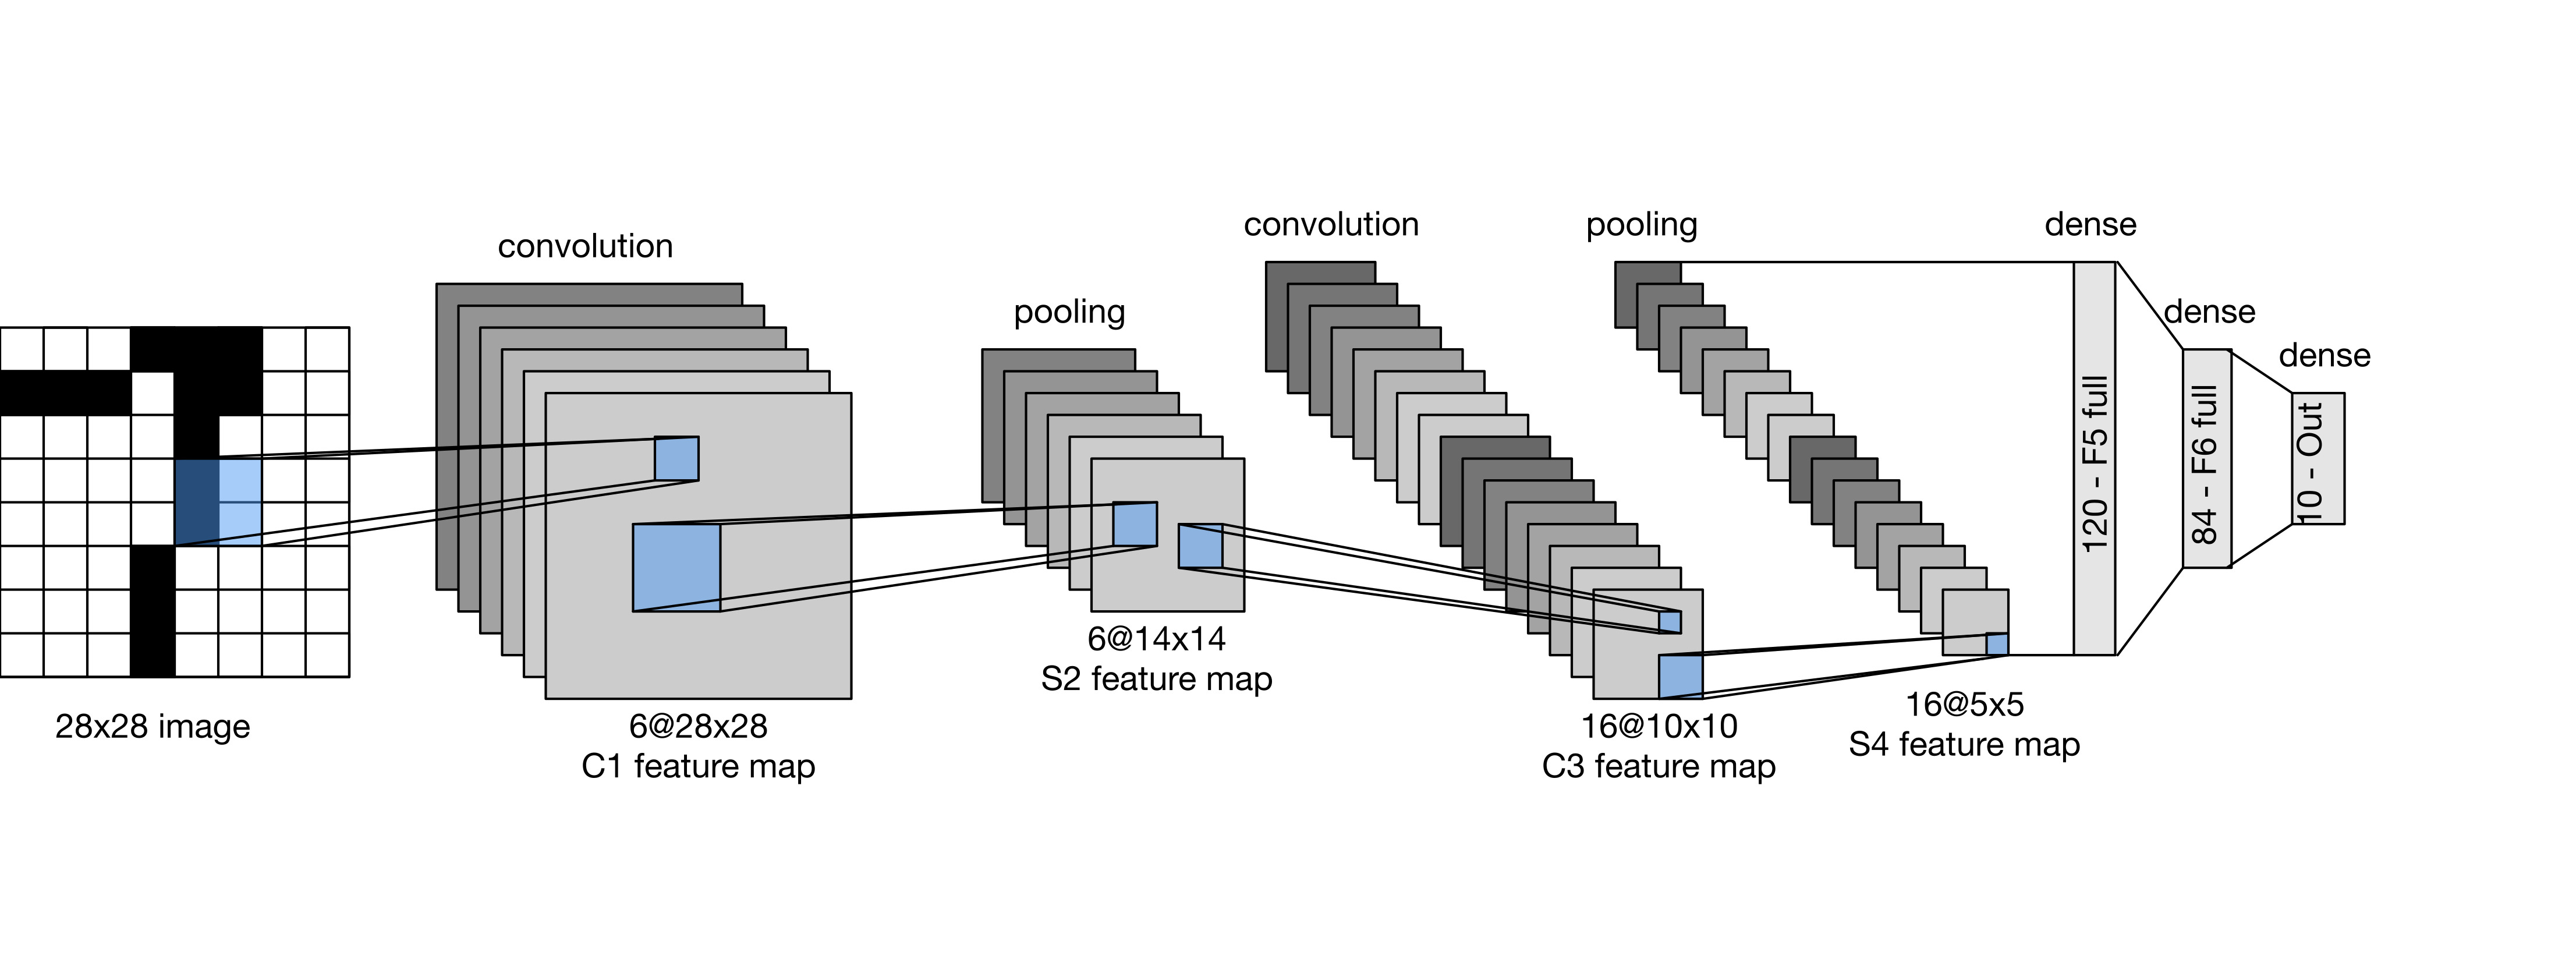
\includegraphics[width=\linewidth, height=5cm, keepaspectratio]{Pictures/convolutional-neural-network/lenet.jpg}
            \caption*{CNN: LeNet \cite{dnn-1}}
        \end{figure}
    \end{minipage}
    \hfill
    \begin{minipage}{0.3\linewidth}
        \begin{figure}[H]
            \centering
            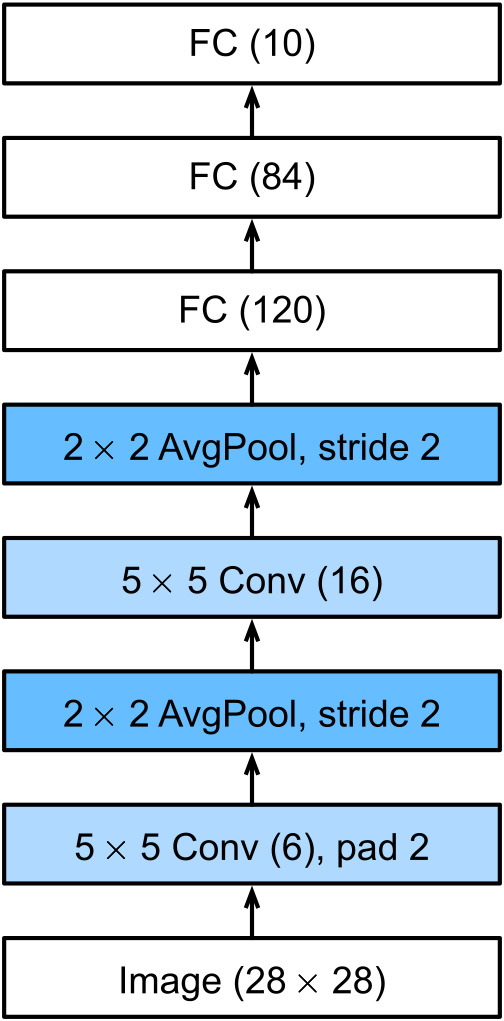
\includegraphics[width=\linewidth, height=5cm, keepaspectratio]{Pictures/convolutional-neural-network/lenet-vert.jpg}
            \caption*{CNN: LeNet \cite{dnn-1}}
        \end{figure}
    \end{minipage}
\end{table}

\begin{enumerate}
    \item LeNet is a convolutional neural network structure proposed by LeCun et al. in 1998. \cite{ieee/726791/cnn-lenet}
    
    
    \item In general, LeNet refers to LeNet-5 and is a simple convolutional neural network.
\end{enumerate}

\begin{lstlisting}[language=Python]
def init_cnn(module):
    """Initialize weights for CNNs."""
    if type(module) == nn.Linear or type(module) == nn.Conv2d:
        nn.init.xavier_uniform_(module.weight)

class LeNet(d2l.Classifier):
    """The LeNet-5 model."""
    def __init__(self, lr=0.1, num_classes=10):
        super().__init__()
        self.save_hyperparameters()
        self.net = nn.Sequential(
            nn.LazyConv2d(6, kernel_size=5, padding=2), nn.Sigmoid(),
            nn.AvgPool2d(kernel_size=2, stride=2),
            nn.LazyConv2d(16, kernel_size=5), nn.Sigmoid(),
            nn.AvgPool2d(kernel_size=2, stride=2),
            nn.Flatten(),
            nn.LazyLinear(120), nn.Sigmoid(),
            nn.LazyLinear(84), nn.Sigmoid(),
            nn.LazyLinear(num_classes))

@d2l.add_to_class(d2l.Classifier)
def layer_summary(self, X_shape):
    X = torch.randn(*X_shape)
    for layer in self.net:
        X = layer(X)
        print(layer.__class__.__name__, 'output shape:\t', X.shape)

model = LeNet()
model.layer_summary((1, 1, 28, 28))
\end{lstlisting}


\begin{lstlisting}[numbers=none]
Conv2d output shape:         torch.Size([1, 6, 28, 28])
Sigmoid output shape:        torch.Size([1, 6, 28, 28])
AvgPool2d output shape:      torch.Size([1, 6, 14, 14])
Conv2d output shape:         torch.Size([1, 16, 10, 10])
Sigmoid output shape:        torch.Size([1, 16, 10, 10])
AvgPool2d output shape:      torch.Size([1, 16, 5, 5])
Flatten output shape:        torch.Size([1, 400])
Linear output shape:         torch.Size([1, 120])
Sigmoid output shape:        torch.Size([1, 120])
Linear output shape:         torch.Size([1, 84])
Sigmoid output shape:        torch.Size([1, 84])
Linear output shape:         torch.Size([1, 10])
\end{lstlisting}







\section{AlexNet (2012) \cite{gfg-convolutional-neural-network-cnn-in-machine-learning, medium/@siddheshb008/alexnet-architecture-explained-b6240c528bd5,wiki-AlexNet,dnn-1}} \label{cnn: AlexNet}

\begin{figure}[H]
    \centering
    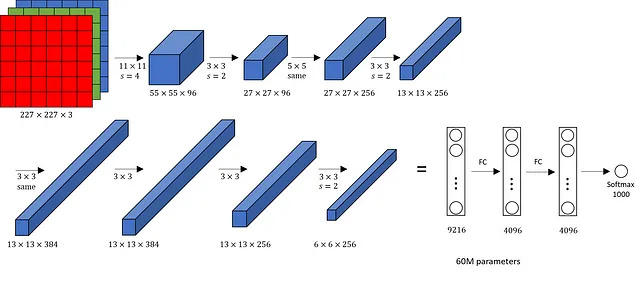
\includegraphics[width=\linewidth, height=5cm, keepaspectratio]{Pictures/convolutional-neural-network/alexnet.jpg}
    \caption*{CNN: AlexNet \cite{dnn-1}}
\end{figure}

\begin{enumerate}
    \item AlexNet is the name of a convolutional neural network (CNN) architecture, designed by \textbf{Alex Krizhevsky} in collaboration with Ilya Sutskever and Geoffrey Hinton, who was Krizhevsky's Ph.D. advisor at the \textbf{University of Toronto}. \cite{wiki-AlexNet}

    \item This was the first architecture that used \textbf{GPU} to boost the training performance.

    \item AlexNet changed the sigmoid activation function to a simpler \textbf{ReLU activation function}

    \item Architecture:\\
    \(
      \displaystyle (\text{CNN} \to \text{RN} \to \text{MP})^{2}\to (\text{CNN}^{3} \to \text{MP})\to (\text{FC} \to \text{DO})^{2} \to \text{Linear}\to \text{softmax}  \hfill \text{\cite{wiki-AlexNet}}
    \)

    \begin{customTableWrapper}{1.3}
    \begin{table}[h]
        \centering
        \begin{tabular}{|l l|}
            \hline
            \customTableHeaderColor
            \textbf{Layer} & \textbf{Description} \\ \hline
            CNN & convolutional layer (with ReLU activation) \\
            RN & local response normalization \\
            MP & maxpooling (SEE: \fullref{cnn: Max Pooling}) \\
            FC & fully connected layer (with ReLU activation) \\
            Linear & fully connected layer (without activation) \\
            DO & dropout \\

            \hline
        \end{tabular}
    \end{table}
    \end{customTableWrapper}
\end{enumerate}

\begin{lstlisting}[language=Python,caption=AlexNet - tensorflow - Python]
class AlexNet(d2l.Classifier):
    def __init__(self, lr=0.1, num_classes=10):
        super().__init__()
        self.save_hyperparameters()
        self.net = tf.keras.models.Sequential([
            tf.keras.layers.Conv2D(filters=96, kernel_size=11, strides=4,
                                   activation='relu'),
            tf.keras.layers.MaxPool2D(pool_size=3, strides=2),
            tf.keras.layers.Conv2D(filters=256, kernel_size=5, padding='same',
                                   activation='relu'),
            tf.keras.layers.MaxPool2D(pool_size=3, strides=2),
            tf.keras.layers.Conv2D(filters=384, kernel_size=3, padding='same',
                                   activation='relu'),
            tf.keras.layers.Conv2D(filters=384, kernel_size=3, padding='same',
                                   activation='relu'),
            tf.keras.layers.Conv2D(filters=256, kernel_size=3, padding='same',
                                   activation='relu'),
            tf.keras.layers.MaxPool2D(pool_size=3, strides=2),
            tf.keras.layers.Flatten(),
            tf.keras.layers.Dense(4096, activation='relu'),
            tf.keras.layers.Dropout(0.5),
            tf.keras.layers.Dense(4096, activation='relu'),
            tf.keras.layers.Dropout(0.5),
            tf.keras.layers.Dense(num_classes)])
AlexNet().layer_summary((1, 224, 224, 1))
\end{lstlisting}

\textbf{Output}:

\begin{lstlisting}[numbers=none]
Conv2D output shape:         (1, 54, 54, 96)
MaxPooling2D output shape:   (1, 26, 26, 96)
Conv2D output shape:         (1, 26, 26, 256)
MaxPooling2D output shape:   (1, 12, 12, 256)
Conv2D output shape:         (1, 12, 12, 384)
Conv2D output shape:         (1, 12, 12, 384)
Conv2D output shape:         (1, 12, 12, 256)
MaxPooling2D output shape:   (1, 5, 5, 256)
Flatten output shape:        (1, 6400)
Dense output shape:  (1, 4096)
Dropout output shape:        (1, 4096)
Dense output shape:  (1, 4096)
Dropout output shape:        (1, 4096)
Dense output shape:  (1, 10)
\end{lstlisting}












\section{VGG-16 (2014) \cite{gfg-convolutional-neural-network-cnn-in-machine-learning,arxiv-1409.1556,gfg-vgg-16-cnn-model,dnn-1}}\label{cnn: VGG-16}

\begin{figure}[H]
    \centering
    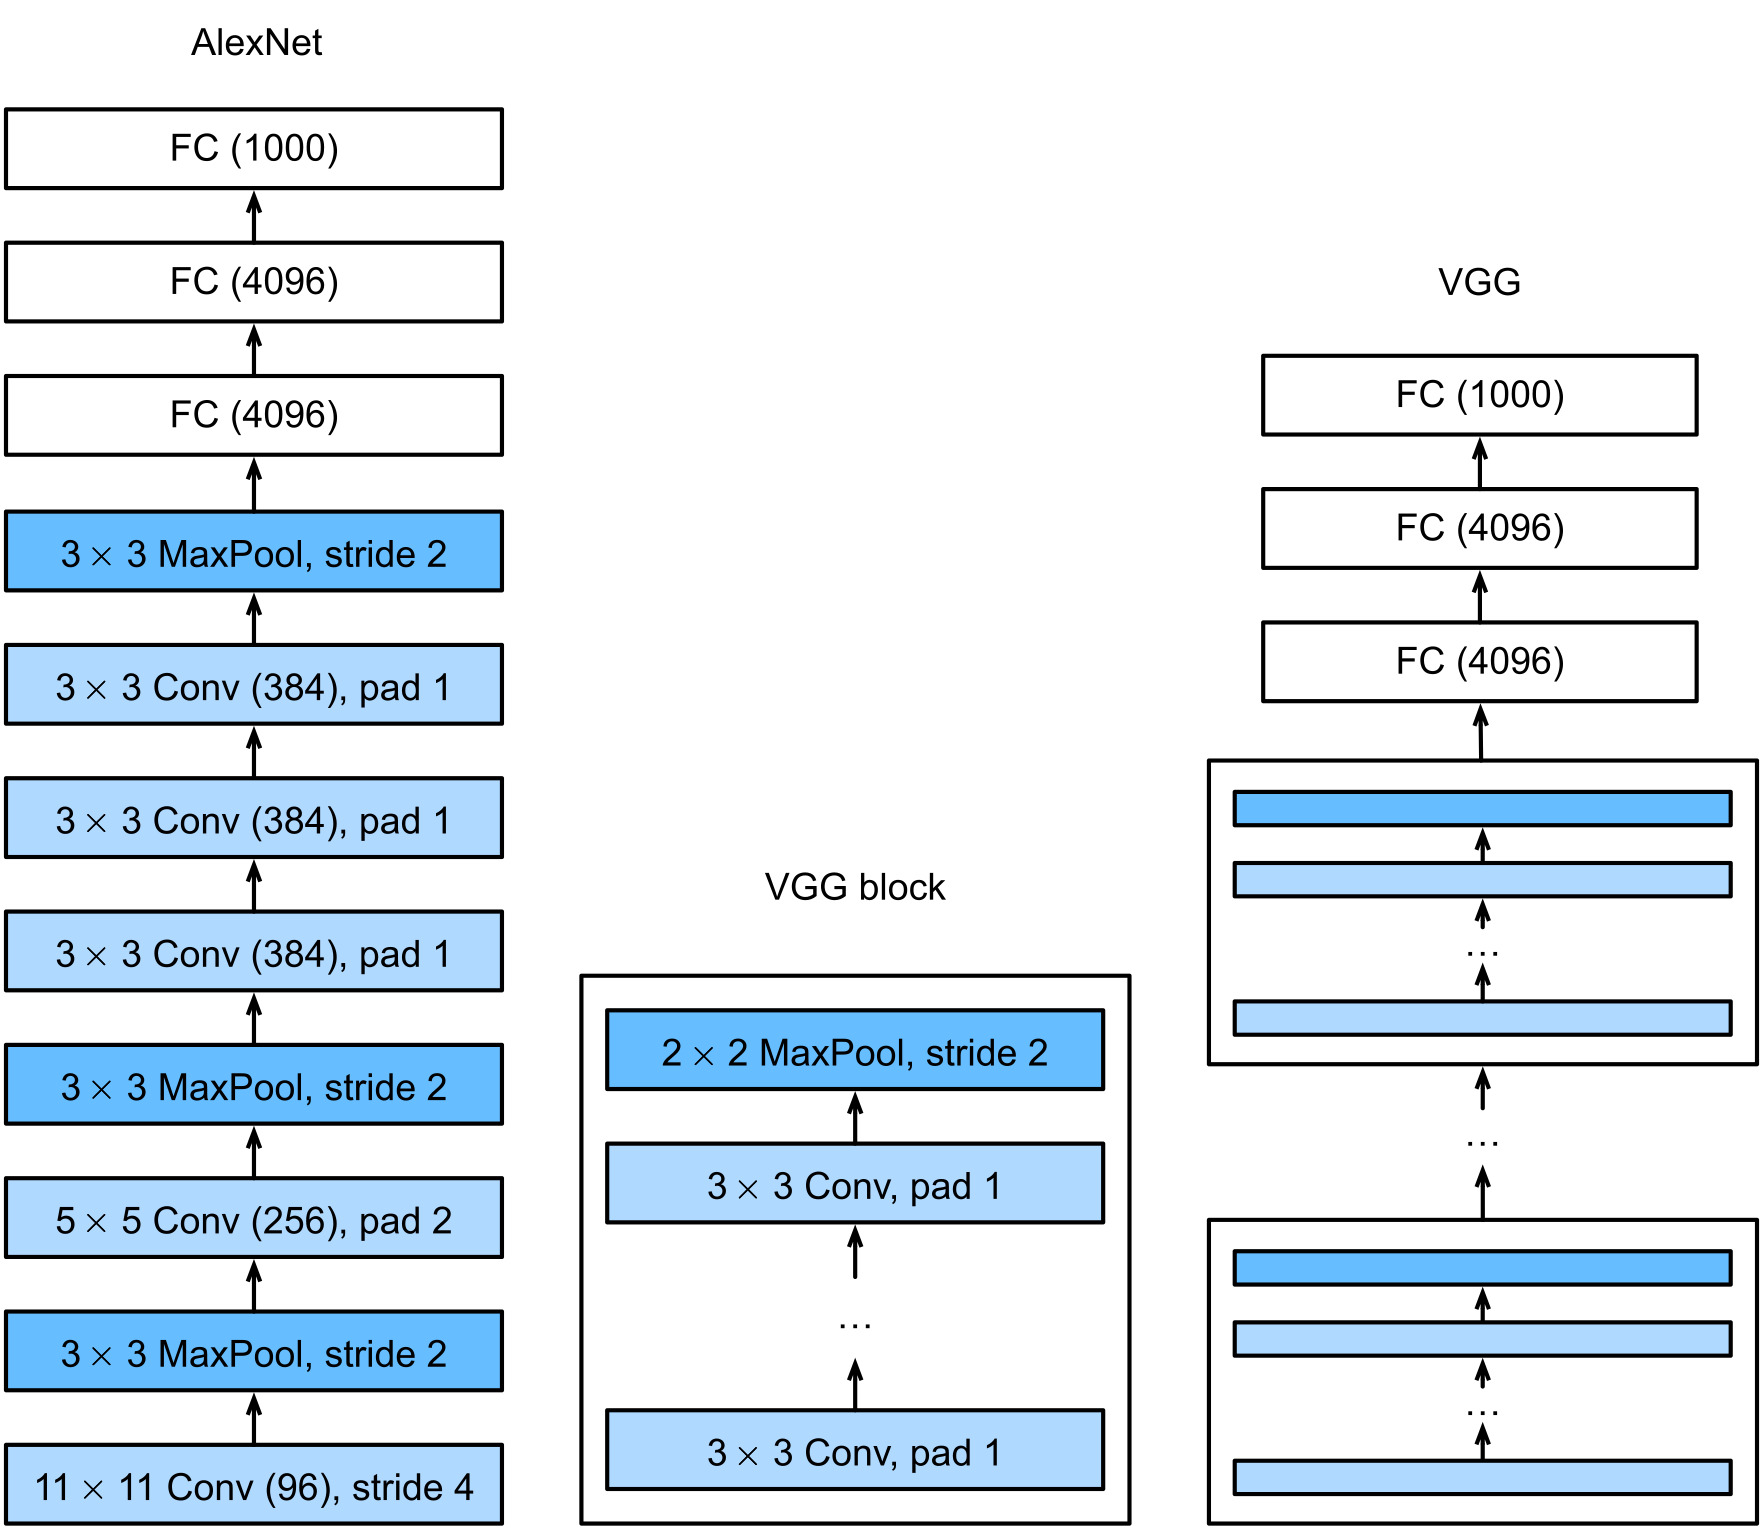
\includegraphics[width=\linewidth, height=7cm, keepaspectratio]{Pictures/convolutional-neural-network/vgg.jpg}
    \caption*{cnn: VGG-16 \cite{dnn-1}}
\end{figure}

\begin{enumerate}
    \item The VGG-16 model is a convolutional neural network (CNN) architecture that was proposed by the \textbf{Visual Geometry Group (VGG)} at the \textbf{University of Oxford}.

    \item The key idea was to use multiple convolutions in between downsampling via max-pooling in the form of a block.

\end{enumerate}

\begin{lstlisting}[language=Python]
def vgg_block(num_convs, out_channels):
    layers = []
    for _ in range(num_convs):
        layers.append(nn.LazyConv2d(out_channels, kernel_size=3, padding=1))
        layers.append(nn.ReLU())
    layers.append(nn.MaxPool2d(kernel_size=2,stride=2))
    return nn.Sequential(*layers)

class VGG(d2l.Classifier):
    def __init__(self, arch, lr=0.1, num_classes=10):
        super().__init__()
        self.save_hyperparameters()
        conv_blks = []
        for (num_convs, out_channels) in arch:
            conv_blks.append(vgg_block(num_convs, out_channels))
        self.net = nn.Sequential(
            *conv_blks, nn.Flatten(),
            nn.LazyLinear(4096), nn.ReLU(), nn.Dropout(0.5),
            nn.LazyLinear(4096), nn.ReLU(), nn.Dropout(0.5),
            nn.LazyLinear(num_classes))
        self.net.apply(d2l.init_cnn)

VGG(arch=((1, 64), (1, 128), (2, 256), (2, 512), (2, 512))).layer_summary(
    (1, 1, 224, 224))
\end{lstlisting}

\begin{lstlisting}[numbers=none]
Sequential output shape:     torch.Size([1, 64, 112, 112])
Sequential output shape:     torch.Size([1, 128, 56, 56])
Sequential output shape:     torch.Size([1, 256, 28, 28])
Sequential output shape:     torch.Size([1, 512, 14, 14])
Sequential output shape:     torch.Size([1, 512, 7, 7])
Flatten output shape:        torch.Size([1, 25088])
Linear output shape:         torch.Size([1, 4096])
ReLU output shape:   torch.Size([1, 4096])
Dropout output shape:        torch.Size([1, 4096])
Linear output shape:         torch.Size([1, 4096])
ReLU output shape:   torch.Size([1, 4096])
Dropout output shape:        torch.Size([1, 4096])
Linear output shape:         torch.Size([1, 10])
\end{lstlisting}






\section*{LeNet, AlexNet, and VGG \cite{dnn-1}}
\begin{enumerate}
    \item all share a common design pattern: extract features exploiting spatial structure via a sequence of convolutions and pooling layers and post-process the representations via fully connected layers.

    \item The improvements upon LeNet by AlexNet and VGG mainly lie in how these later networks widen and deepen these two modules.

    
\end{enumerate}


\subsection*{major challenges \cite{dnn-1}}
\begin{enumerate}
    \item the fully connected layers at the end of the architecture consume tremendous numbers of parameters

    \item it is equally impossible to add fully connected layers earlier in the network to increase the degree of nonlinearity: doing so would destroy the spatial structure and require potentially even more memory

\end{enumerate}






\section{Network In Network (NiN) (2013) \cite{arxiv/1312.4400-nin,medium/towardsdatascience.com/review-nin-network-in-network-image-classification-69e271e499ee,dnn-1}}\label{Network In Network (NiN)}

\begin{figure}[H]
    \centering
    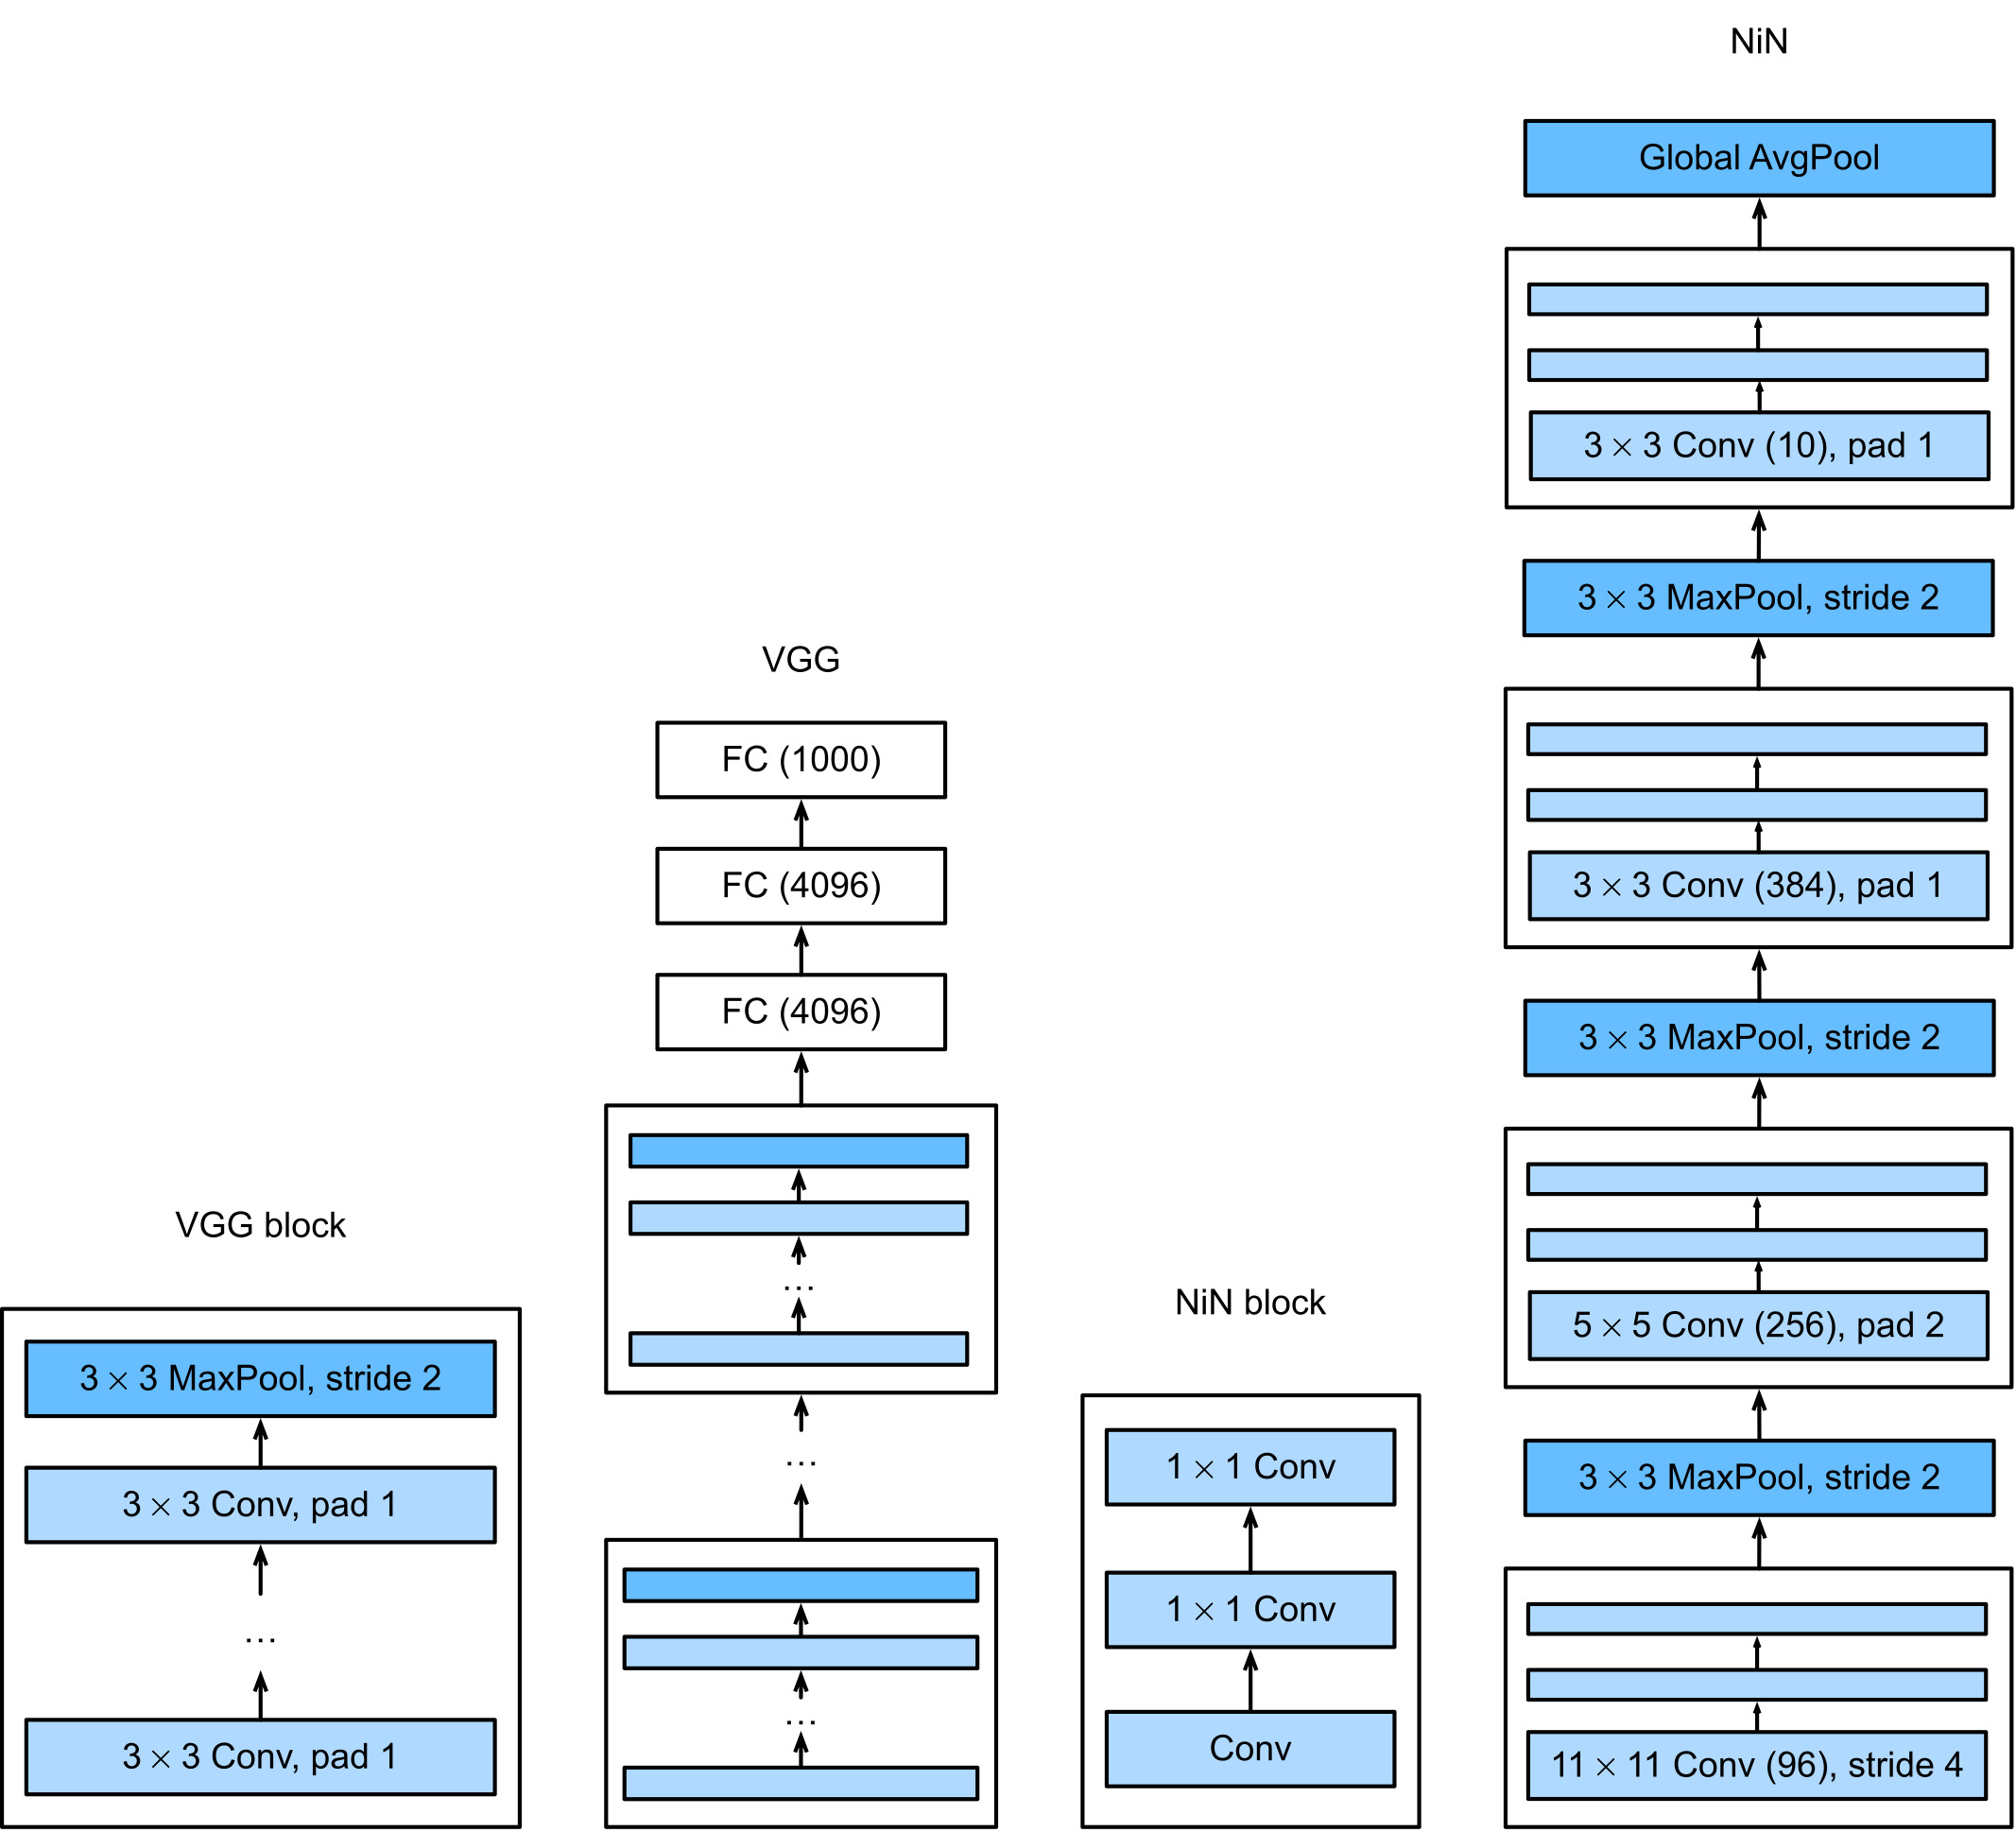
\includegraphics[width=\linewidth, height=6.5cm, keepaspectratio]{Pictures/convolutional-neural-network/nin.jpg}
\end{figure}


\begin{enumerate}[itemsep=0.2cm]
    \item They were proposed based on a very simple insight: 
    \begin{enumerate}
        \item use $1\times 1$ convolutions to add local nonlinearities across the channel activations 
        \item use global average pooling to integrate across all locations in the last representation layer. 
    \end{enumerate}
    
    \item Note that global average pooling would not be effective, were it not for the added nonlinearities. 

\end{enumerate}


\begin{lstlisting}[language=Python]
def nin_block(out_channels, kernel_size, strides, padding):
    return nn.Sequential(
        nn.LazyConv2d(out_channels, kernel_size, strides, padding), nn.ReLU(),
        nn.LazyConv2d(out_channels, kernel_size=1), nn.ReLU(),
        nn.LazyConv2d(out_channels, kernel_size=1), nn.ReLU())

class NiN(d2l.Classifier):
    def __init__(self, lr=0.1, num_classes=10):
        super().__init__()
        self.save_hyperparameters()
        self.net = nn.Sequential(
            nin_block(96, kernel_size=11, strides=4, padding=0),
            nn.MaxPool2d(3, stride=2),
            nin_block(256, kernel_size=5, strides=1, padding=2),
            nn.MaxPool2d(3, stride=2),
            nin_block(384, kernel_size=3, strides=1, padding=1),
            nn.MaxPool2d(3, stride=2),
            nn.Dropout(0.5),
            nin_block(num_classes, kernel_size=3, strides=1, padding=1),
            nn.AdaptiveAvgPool2d((1, 1)),
            nn.Flatten())
        self.net.apply(d2l.init_cnn)

NiN().layer_summary((1, 1, 224, 224))
\end{lstlisting}

\begin{lstlisting}[numbers=none]
Sequential output shape:     torch.Size([1, 96, 54, 54])
MaxPool2d output shape:      torch.Size([1, 96, 26, 26])
Sequential output shape:     torch.Size([1, 256, 26, 26])
MaxPool2d output shape:      torch.Size([1, 256, 12, 12])
Sequential output shape:     torch.Size([1, 384, 12, 12])
MaxPool2d output shape:      torch.Size([1, 384, 5, 5])
Dropout output shape:        torch.Size([1, 384, 5, 5])
Sequential output shape:     torch.Size([1, 10, 5, 5])
AdaptiveAvgPool2d output shape:      torch.Size([1, 10, 1, 1])
Flatten output shape:        torch.Size([1, 10])
\end{lstlisting}








\section{Multi-Branch Networks (GoogLeNet) (2015) \cite{arxiv/1409.4842-googlenet,dnn-1}} \label{Multi-Branch Networks (GoogLeNet)}

\begin{table}[H]
    \begin{minipage}{0.45\linewidth}
        \begin{figure}[H]
            \centering
            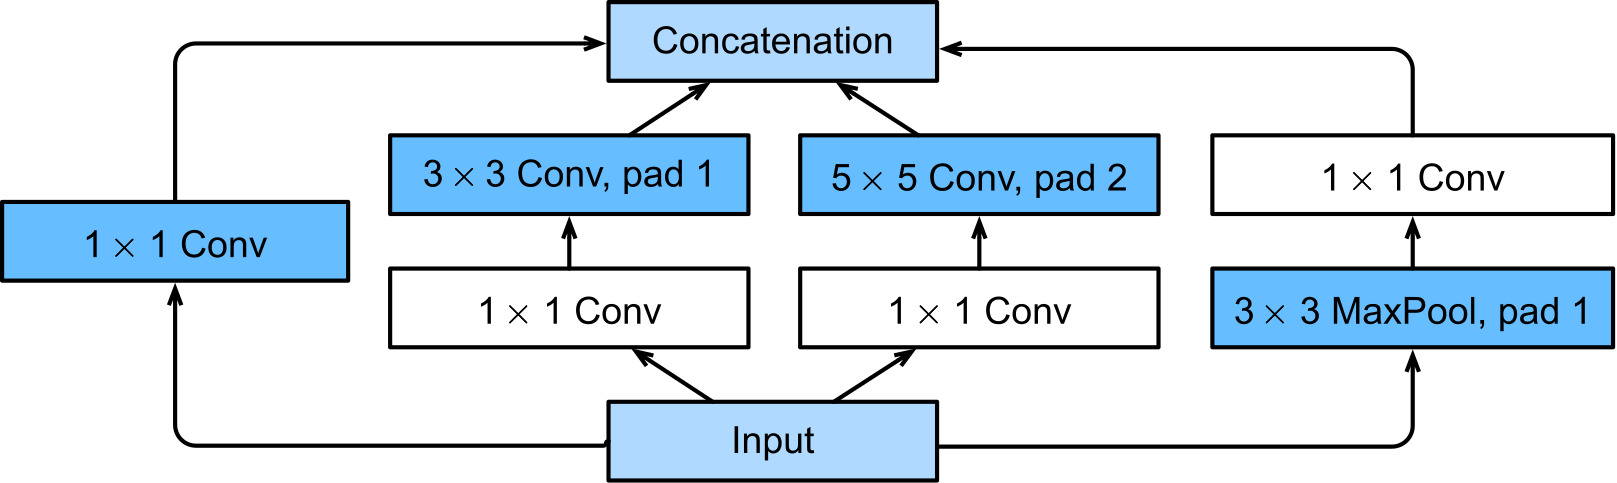
\includegraphics[width=\linewidth, height=3.5cm, keepaspectratio]{Pictures/convolutional-neural-network/inception-block.jpg}
            \caption*{Inception Block}
        \end{figure}
    \end{minipage}
    \hfill
    \begin{minipage}{0.45\linewidth}
        \begin{figure}[H]
            \centering
            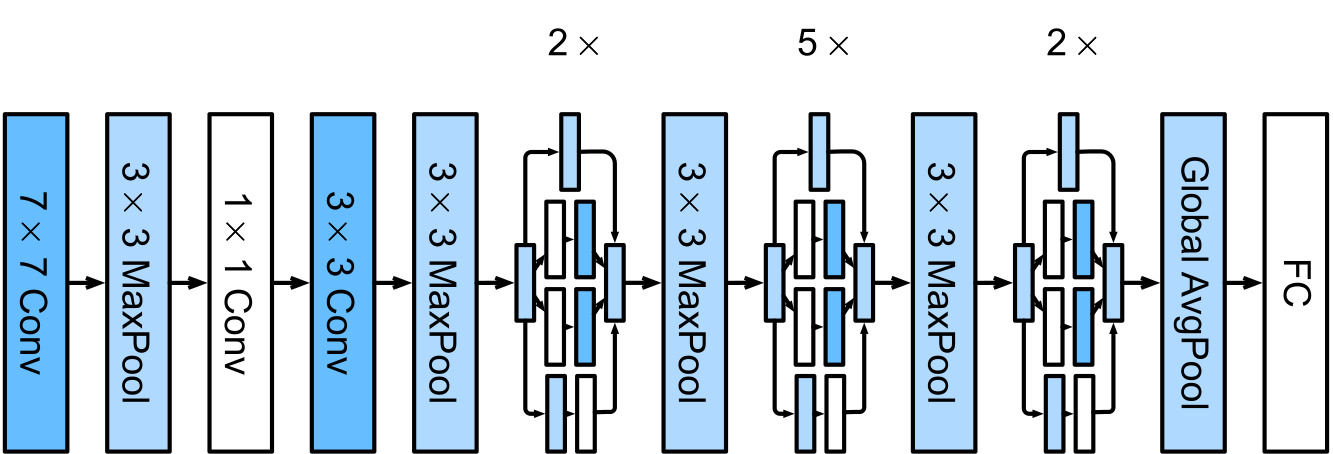
\includegraphics[width=\linewidth, height=3.5cm, keepaspectratio]{Pictures/convolutional-neural-network/inception-full-90-googlenet.jpg}
            \caption*{GoogleNet}
        \end{figure}
    \end{minipage}
\end{table}

\subsection{Inception Blocks \cite{dnn-1}} \label{Inception Blocks}

\begin{enumerate}[itemsep=0.1cm]
    \item the inception block consists of four \textbf{parallel branches}
    \begin{enumerate}
        \item The first three branches use convolutional layers with window sizes of $1\times 1$, $3\times 3$, and $5\times 5$ to extract information from different spatial sizes. 
        
        \item The middle two branches also add a $1\times 1$ convolution of the input to reduce the number of channels, reducing the model’s complexity. 
        
        \item The fourth branch uses a $3\times 3$ max-pooling layer, followed by a $1\times 1$ convolutional layer to change the number of channels.

    \end{enumerate}

    \item The four branches all use appropriate padding to give the input and output the same height and width. 

    \item Finally, the outputs along each branch are concatenated along the channel dimension and comprise the block’s output. 

    \item The commonly-tuned hyper-parameters of the Inception block are the number of output channels per layer, i.e., how to allocate capacity among convolutions of different size.

    \item To gain some intuition for why this network works so well, consider the combination of the filters. They explore the image in a variety of filter sizes.\\
    This means that details at different extents can be recognized efficiently by filters of different sizes.\\
    At the same time, we can allocate different amounts of parameters for different filters.

\end{enumerate}


\subsection{GoogLeNet Model \cite{dnn-1}}

\begin{enumerate}
    \item GoogLeNet uses a stack of a total of 9 inception blocks, arranged into three groups with max-pooling in between, and global average pooling in its head to generate its estimates. 
    
    \item Max-pooling between inception blocks reduces the dimensionality.

    \item At its stem, the first module is similar to AlexNet and LeNet.

    \item The GoogLeNet model is computationally complex. 
    
    \item Note the large number of relatively arbitrary hyperparameters in terms of the number of channels chosen, the number of blocks prior to dimensionality reduction, the relative partitioning of capacity across channels, etc.

    
\end{enumerate}



\section{Residual Networks (ResNet) \cite{dnn-1}} \label{Residual Networks (ResNet)}

SEE: \fullref{nn: Function Classes}

\begin{table}[H]
    \begin{minipage}[b]{0.4\linewidth}
        \begin{figure}[H]
            \centering
            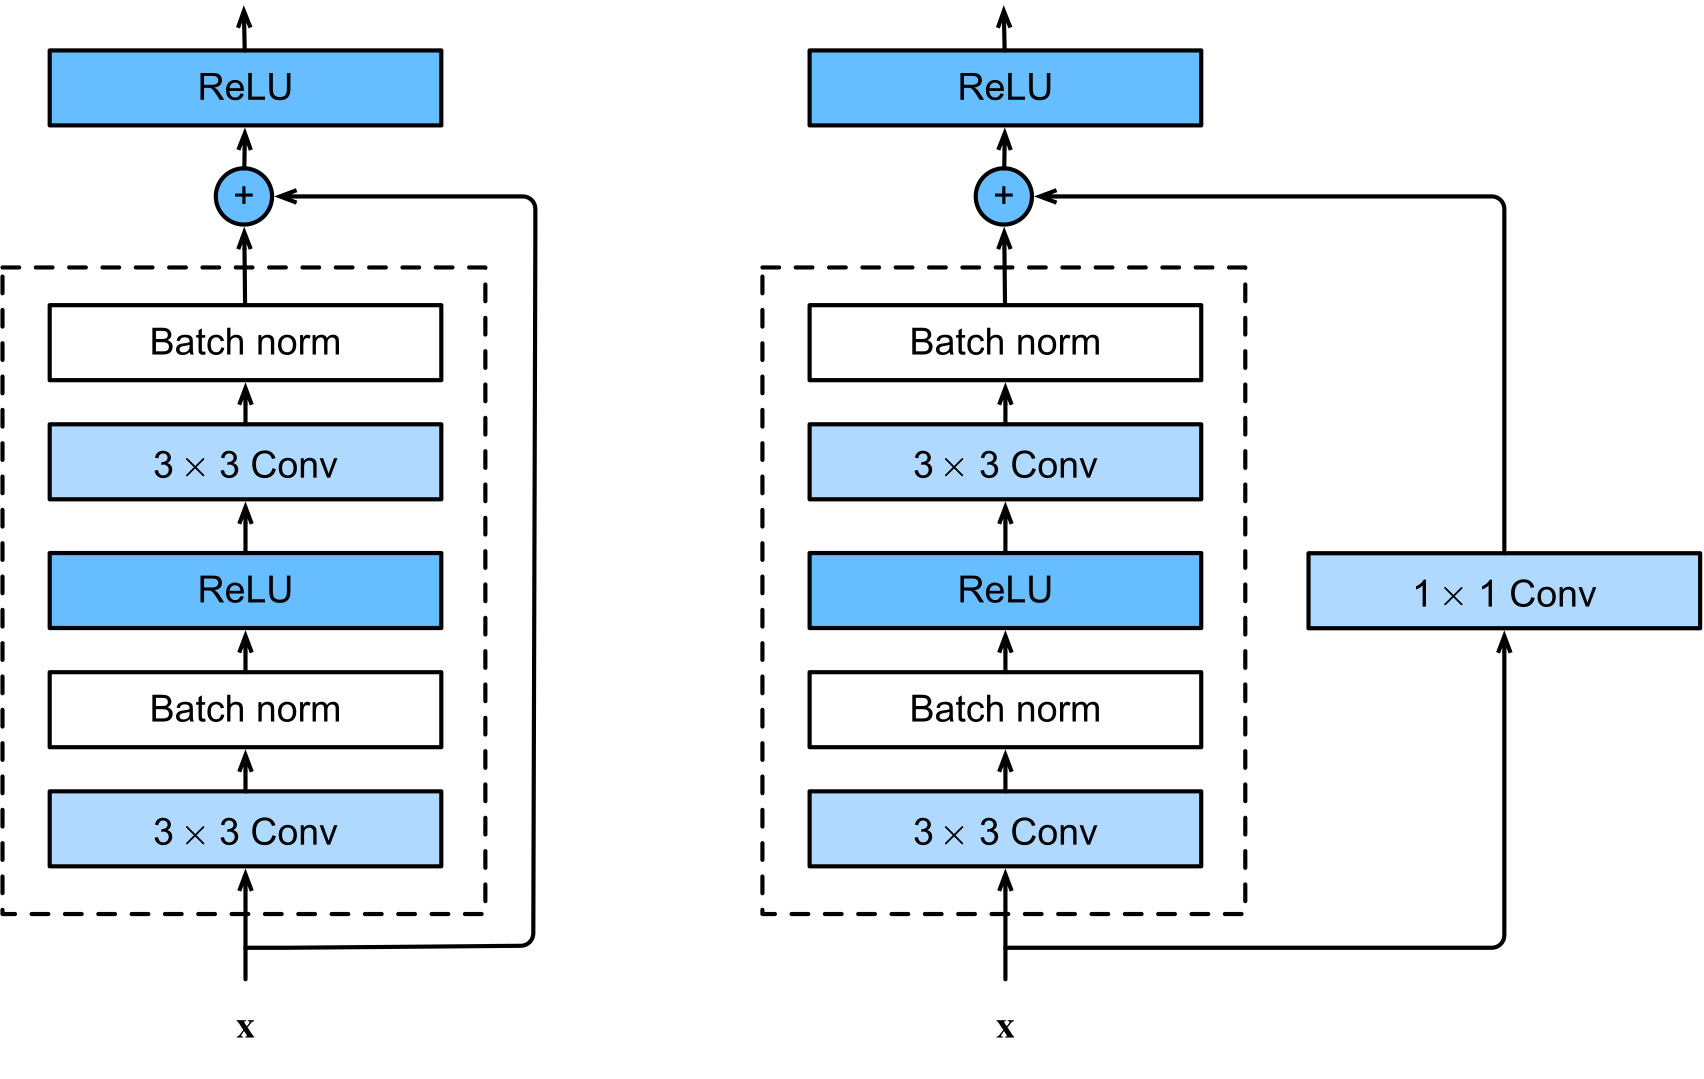
\includegraphics[width=\linewidth, height=4cm, keepaspectratio]{Pictures/convolutional-neural-network/resnet-block.jpg}
            \caption{Resnet Block}
        \end{figure}
    \end{minipage}
    \hfill
    \begin{minipage}[b]{0.55\linewidth}
        \begin{figure}[H]
            \centering
            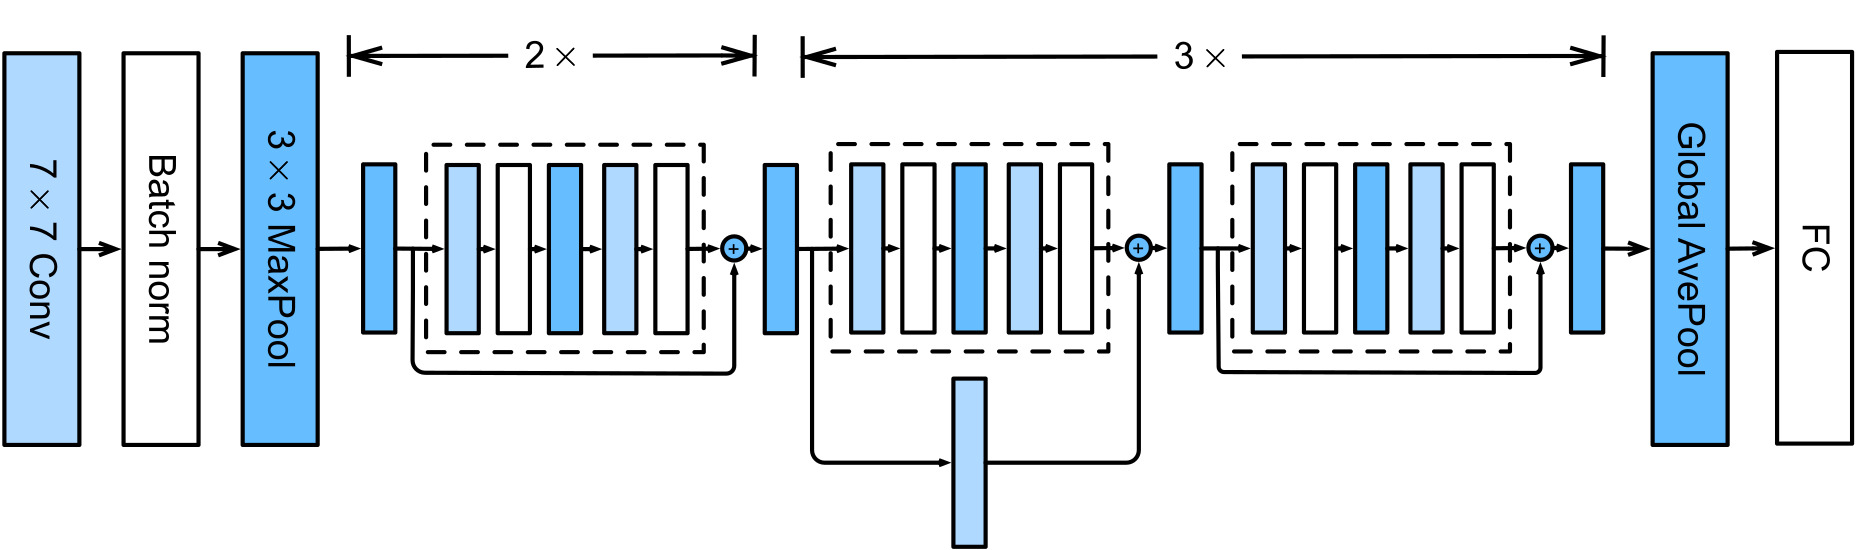
\includegraphics[width=\linewidth, height=4cm, keepaspectratio]{Pictures/convolutional-neural-network/resnet18-90.jpg}
            \caption{ResNet-18 architecture}
        \end{figure}
    \end{minipage}
\end{table}

\begin{enumerate}
    \item if we can train the newly-added layer into an identity function $f(\mathbf{x}) = \mathbf{x}$, the new model will be as effective as the original model. As the new model may get a better solution to fit the training dataset, the added layer might make it easier to reduce training errors.

    \item At the heart of the proposed residual network (ResNet) is the idea that every additional layer should more easily contain the identity function as one of its elements. 
    
    \item The considerations are rather profound but they led to a surprisingly simple solution, a residual block.

    
\end{enumerate}



\subsection{Residual Block \cite{dnn-1}} \label{Residual Block}

\begin{table}[H]
    \begin{minipage}{0.25\linewidth}
        \begin{figure}[H]
            \centering
            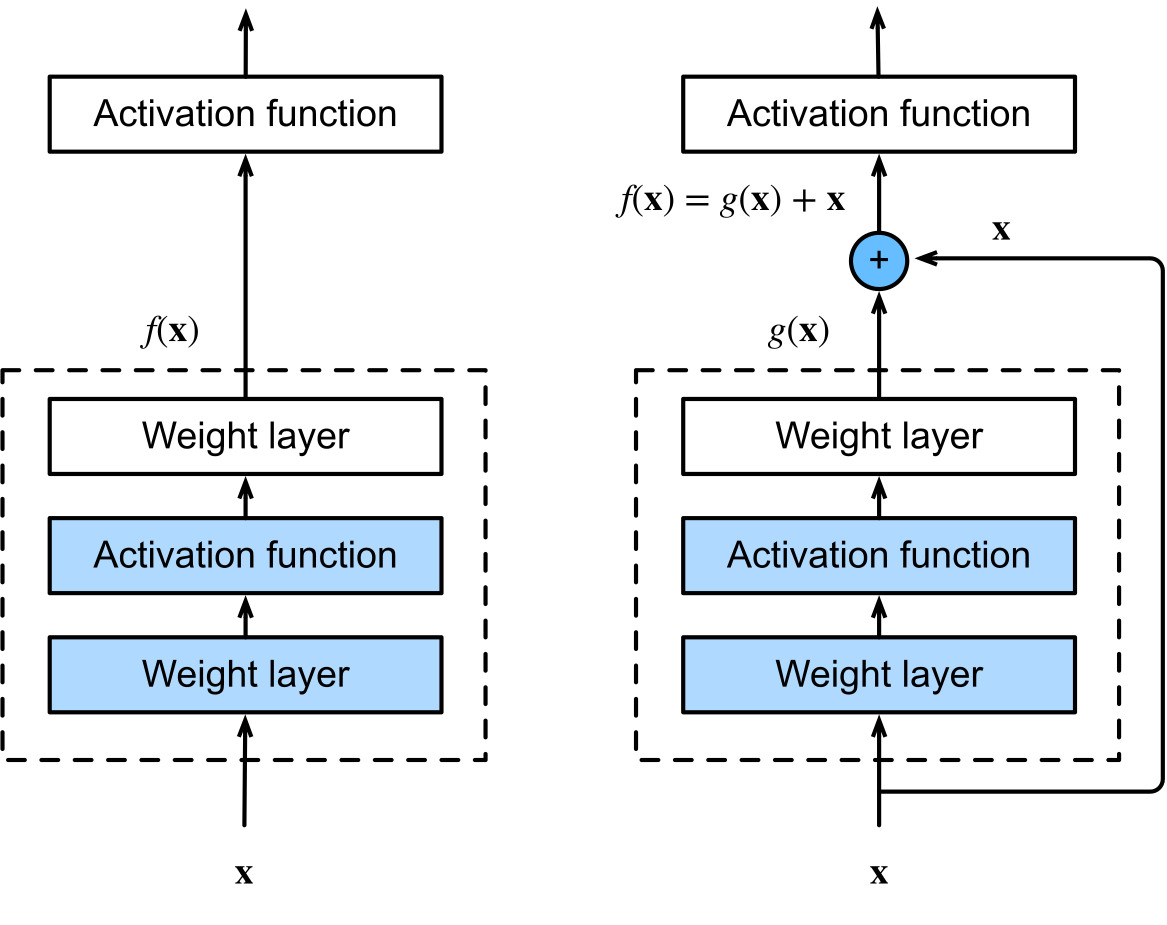
\includegraphics[width=\linewidth, height=4cm, keepaspectratio]{Pictures/convolutional-neural-network/residual-block.jpg}
            \caption{Residual Block}
        \end{figure}
    \end{minipage}
    \hfill
    \begin{minipage}{0.7\linewidth}
        \begin{customTableWrapper}{1.3}
            \begin{table}[H]
                \centering
                \begin{tabular}{l p{6cm}}
                    $\mathbf{x}$ & input \\
                    $f(\mathbf{x})$ & desired underlying mapping we want to obtain by learning\\
                    $g(\mathbf{x}) = f(\mathbf{x}) - \mathbf{x}$ & residual mapping
                \end{tabular}
            \end{table}
        \end{customTableWrapper}
    \end{minipage}
\end{table}

\begin{enumerate}
    \item If the identity mapping $f(\mathbf{x}) = \mathbf{x}$ is the desired underlying mapping, the residual mapping amounts to $g(\mathbf{x}) = 0$ and it is thus easier to learn: we only need to push the weights and biases of the upper weight layer (e.g., fully connected layer and convolutional layer) within the dotted-line box to zero.

    \item he right figure illustrates the residual block of ResNet, where the solid line carrying the layer input $\mathbf{x}$ to the addition operator is called a \textbf{residual connection}\indexlabel{residual connection} (or \textit{shortcut connection}). 
    
    \item With residual blocks, inputs can forward propagate faster through the residual connections across layers. 
    
    \item The residual block can be thought of as a \textbf{special case of the multi-branch Inception block}: it has two branches one of which is the identity mapping.

    \item One of the \textbf{challenges} one encounters in the design of ResNet is the trade-off between nonlinearity and dimensionality within a given block.\\
    That is, we could add more nonlinearity by increasing the number of layers, or by increasing the width of the convolutions.\\
    An alternative strategy is to increase the number of channels that can carry information between blocks. Unfortunately, the latter comes with a quadratic penalty since the computational cost of ingesting $c_i$ channels and emitting $c_o$ channels is proportional to $\mathcal{O}(c_\textrm{i} \cdot c_\textrm{o})$
\end{enumerate}






\section{ResNeXt \cite{dnn-1}} \label{ResNeXt}

\begin{figure}[H]
    \centering
    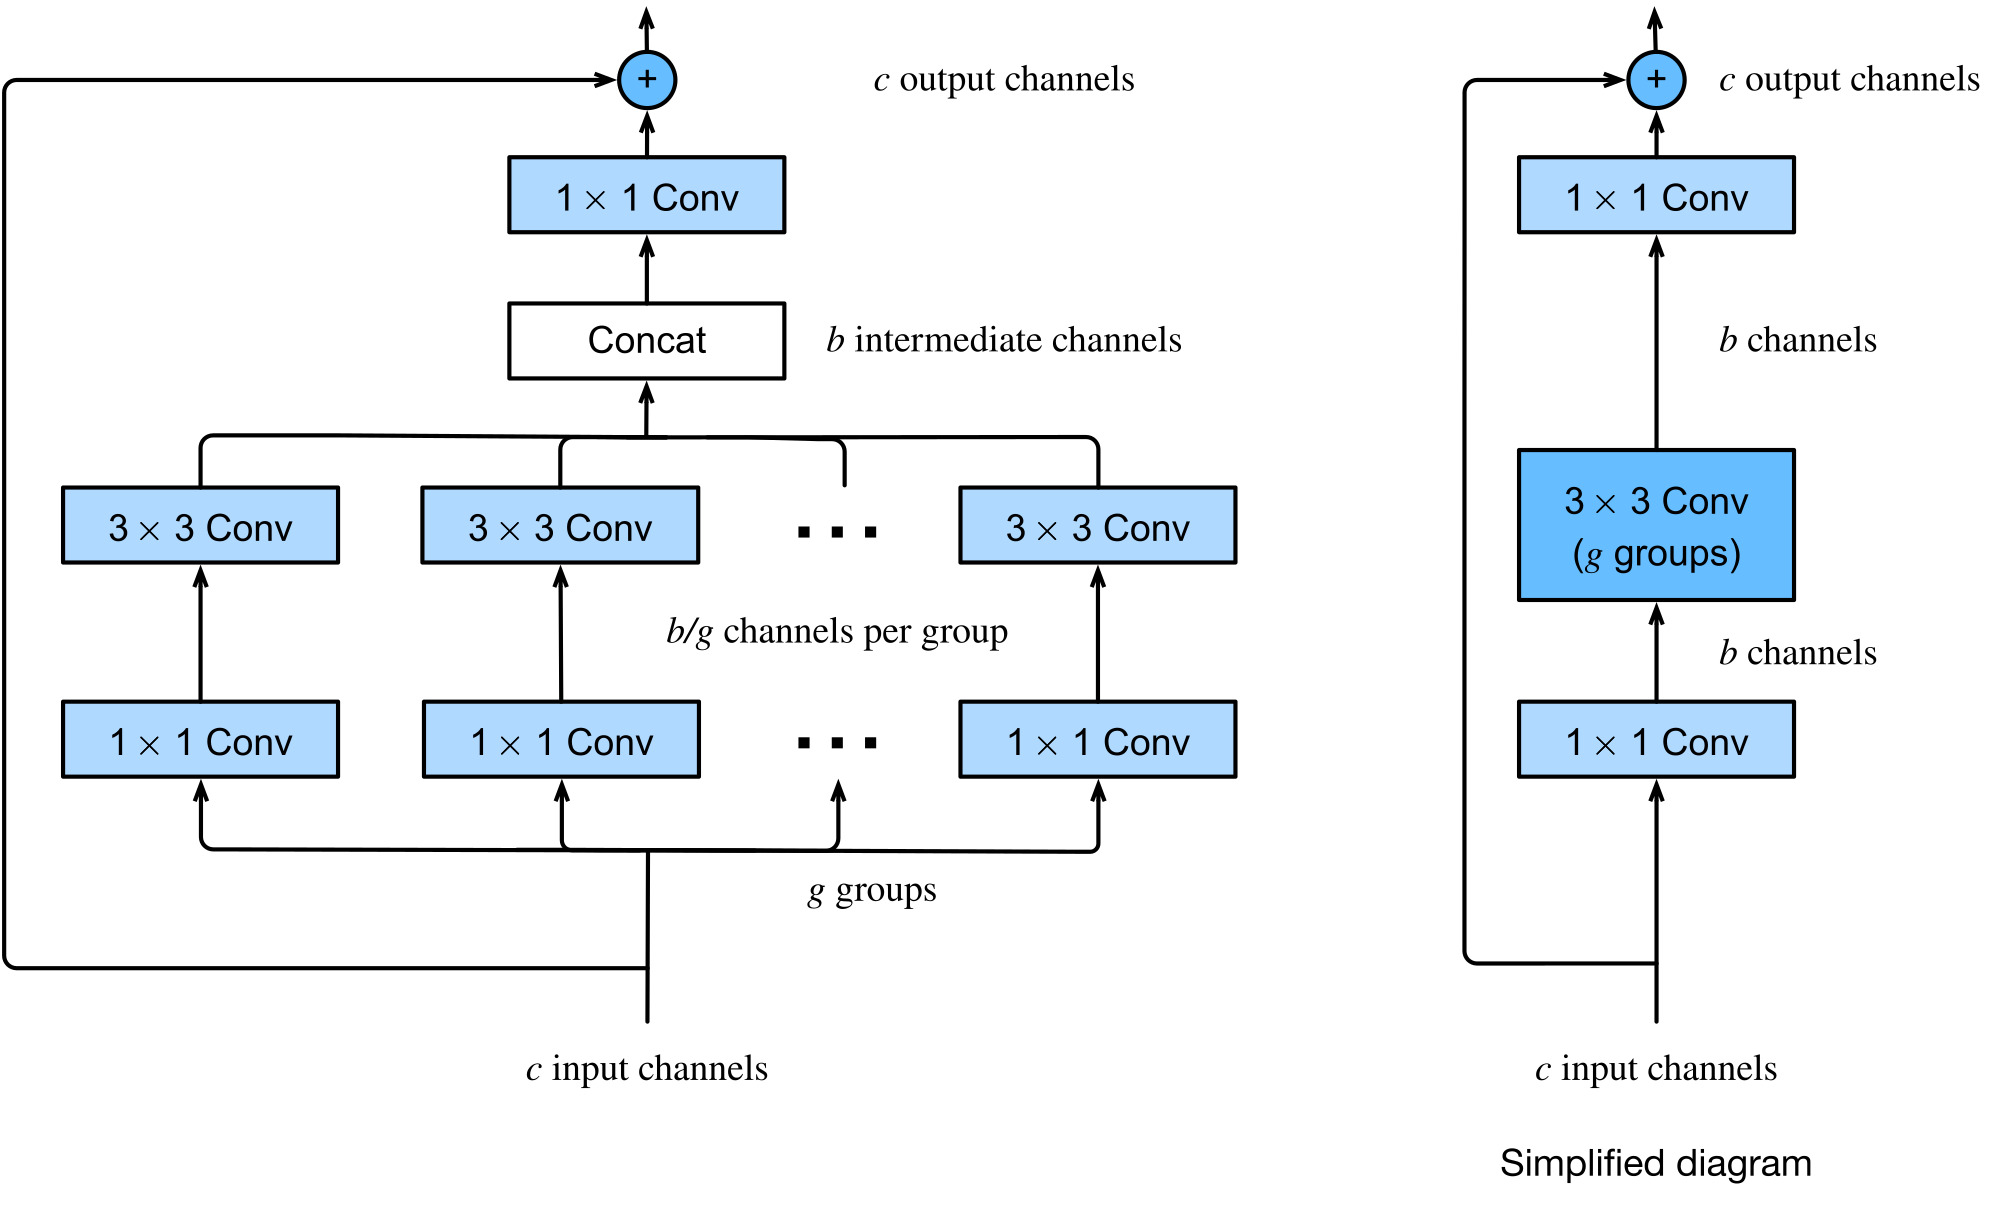
\includegraphics[width=\linewidth, height=5cm, keepaspectratio]{Pictures/convolutional-neural-network/resnext-block.jpg}
    \caption{Resnext Block}
\end{figure}


\begin{enumerate}
    \item Applying the idea of \textbf{multiple independent groups} to the ResNet block led to the design of ResNeXt. 
    
    \item Different from the smorgasbord of transformations in Inception, ResNeXt adopts the same transformation in all branches, thus minimizing the need for manual tuning of each branch.

    \item Breaking up a convolution from $c_i$ to $c_o$ channels into one of $g$ groups of size $c_i/g$ generating $g$ outputs of size $c_o/g$ is called, quite fittingly, a \textbf{grouped convolution} \indexlabel{grouped convolution}.

    \item The computational cost (proportionally) is reduced from $\mathcal{O}(c_\textrm{i} \cdot c_\textrm{o})$ to $\mathcal{O}(g \cdot (c_\textrm{i}/g) \cdot (c_\textrm{o}/g)) = \mathcal{O}(c_\textrm{i} \cdot c_\textrm{o} / g)$, i.e., it is $g$ times faster.

    \item Even better, the number of parameters needed to generate the output is also reduced from a $c_\textrm{i} \times c_\textrm{o}$ matrix to $g$ smaller matrices of size $(c_\textrm{i}/g) \times (c_\textrm{o}/g)$, again a $g$ times reduction.

    \item we assume that both $c_i$ and $c_o$ are divisible by $g$.

    \item The only challenge in this design is that no information is exchanged between the $g$ groups\\
    The ResNeXt block of Fig. 8.6.5 amends this in two ways:
    \begin{enumerate}
        \item the grouped convolution with a $3 \times 3$ kernel is sandwiched in between two $1 \times 1$ convolutions

        \item The second one serves double duty in changing the number of channels back

        \item The benefit is that we only pay the $\mathcal{O}(c \cdot b)$ cost for $1 \times 1$ kernels and can make do with an $\mathcal{O}(b^2 / g)$ cost for $3 \times 3$ kernels

    \end{enumerate}
\end{enumerate}









\section{Densely Connected Networks (DenseNet) \cite{dnn-1}} \label{Densely Connected Networks (DenseNet)}


\begin{table}[H]
    \begin{minipage}{0.48\linewidth}
        \begin{figure}[H]
            \centering
            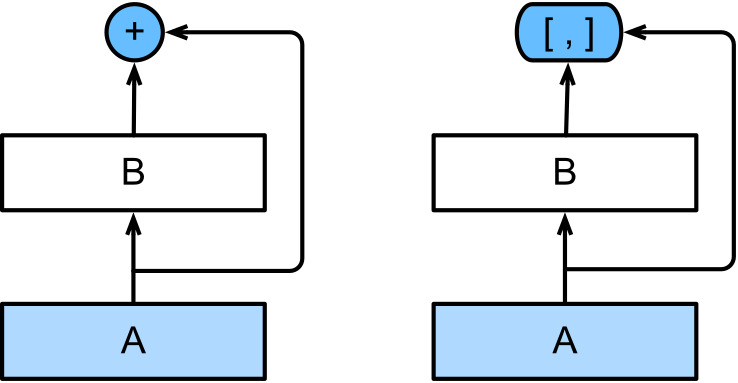
\includegraphics[width=\linewidth, height=2cm, keepaspectratio]{Pictures/convolutional-neural-network/densenet-block.jpg}
            \caption{DenseNet Block}
        \end{figure}
    \end{minipage}
    \hfill
    \begin{minipage}{0.48\linewidth}
        \begin{figure}[H]
            \centering
            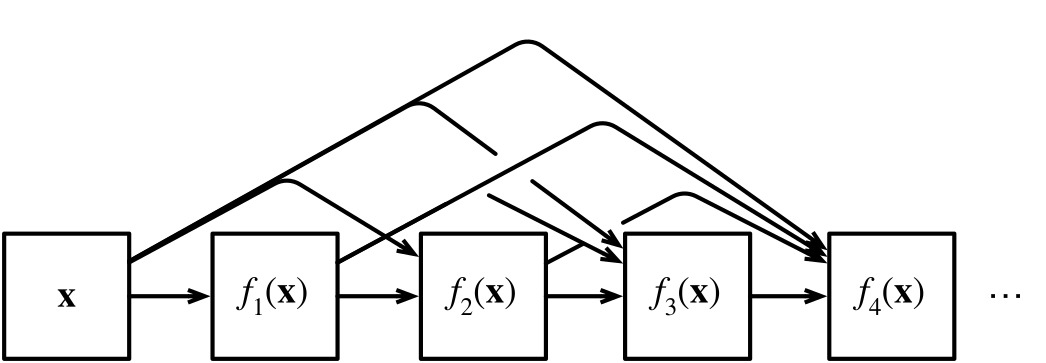
\includegraphics[width=\linewidth, height=2cm, keepaspectratio]{Pictures/convolutional-neural-network/densenet.jpg}
            \caption{DenseNet}
        \end{figure}
    \end{minipage}
\end{table}


\begin{enumerate}[itemsep=0.2cm]
    \item DenseNet is characterized by both\\
    the \textbf{connectivity pattern} where each layer connects to all the preceding layers and\\
    the concatenation operation (rather than the addition operator in ResNet) to preserve and reuse features from earlier layers.

    \item Taylor expansion for functions At the point $x = 0$ :
    \[
        \hfill
        f(x) = f(0) + x \cdot \left[f'(0) + x \cdot \left[\frac{f''(0)}{2!}  + x \cdot \left[\frac{f'''(0)}{3!}  + \cdots \right]\right]\right]
        \hfill
    \]

    \item the key difference between ResNet and DenseNet is that in the latter case outputs are concatenated (denoted by $[,\;]$) rather than added. As a result, we perform a mapping from $\mathbf{x}$ to its values after applying an increasingly complex sequence of functions:
    \[
        \hfill
        \mathbf{x} \to \left[
        \mathbf{x},
        f_1(\mathbf{x}),
        f_2\left(\left[\mathbf{x}, f_1\left(\mathbf{x}\right)\right]\right), f_3\left(\left[\mathbf{x}, f_1\left(\mathbf{x}\right), f_2\left(\left[\mathbf{x}, f_1\left(\mathbf{x}\right)\right]\right)\right]\right), \ldots\right]
        \hfill
    \]

    \item In the end, all these functions are combined in MLP to reduce the number of features again.
    
    \item In terms of implementation this is quite simple: rather than adding terms, we concatenate them.
    
    \item The name DenseNet arises from the fact that the dependency graph between variables becomes quite dense. 
    
    \item The final layer of such a chain is densely connected to all previous layers.

    \item The main components that comprise a DenseNet are:
    \begin{enumerate}
        \item \textbf{dense blocks}: define how the inputs and outputs are concatenated
        
        \item \textbf{transition layers}: control the number of channels so that it is not too large, since the expansion $\mathbf{x} \to \left[\mathbf{x}, f_1(\mathbf{x}), f_2\left(\left[\mathbf{x}, f_1\left(\mathbf{x}\right)\right]\right), \ldots \right]$ can be quite high-dimensional.
    \end{enumerate}
\end{enumerate}

\subsection{Dense Block \cite{dnn-1}}

\begin{enumerate}
    \item DenseNet uses the modified “batch normalization, activation, and convolution” structure of ResNet

    \item A dense block consists of multiple convolution blocks, each using the same number of output channels. 
    
    \item In the forward propagation, however, we concatenate the input and output of each convolution block on the channel dimension.

    \item The number of convolution block channels controls the growth in the number of output channels relative to the number of input channels. This is also referred to as the \textbf{growth rate}.
\end{enumerate}


\subsection{Transition Layers \cite{dnn-1}}

\begin{enumerate}
    \item Since each dense block will increase the number of channels, adding too many of them will lead to an excessively complex model. A transition layer is used to control the complexity of the model. It reduces the number of channels by using a $1 \times 1$ convolution. 
    
    \item Moreover, it halves the height and width via average pooling with a stride of $2$.



\end{enumerate}












\section{Region Based CNNs (R-CNN/ RCNN) (2013) \cite{arxiv-1311.2524v5-rcnn,https://www.geeksforgeeks.org/r-cnn-region-based-cnns/}}\label{Region Based CNNs (R-CNN/ RCNN)}

\begin{figure}[H]
    \centering
    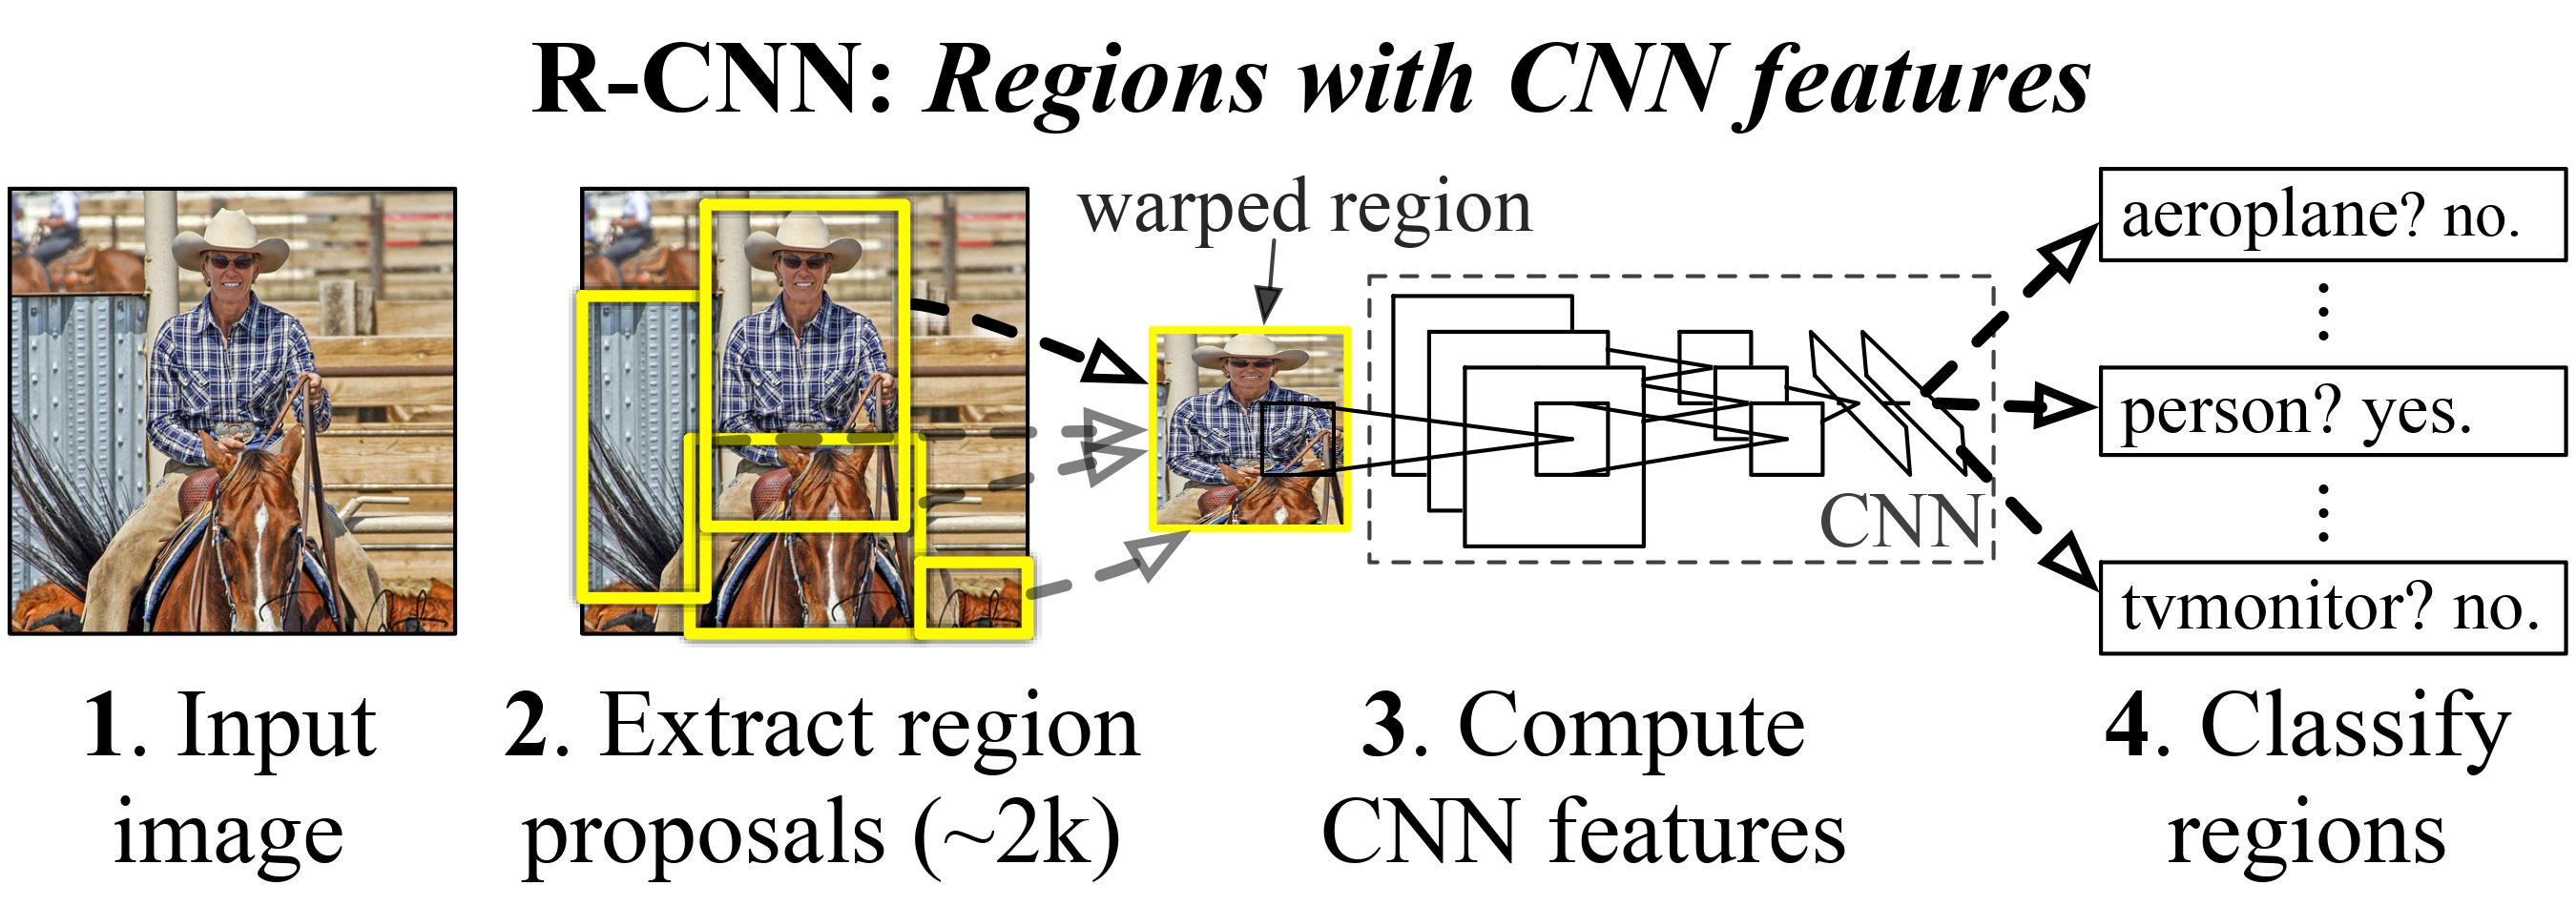
\includegraphics[width=\linewidth, height=3.5cm, keepaspectratio]{Pictures/convolutional-neural-network/rcnn-splash-method.jpg}
    \caption*{R-CNN}
\end{figure}

\begin{enumerate}
    \item Convolution Neural Network (CNN) with a fully connected layer is \textbf{NOT} able to deal with the frequency of occurrence and multi objects.

    \item We can use a sliding window brute force search to select a region and apply the CNN model to that.\\
    \textbf{Disadvantages}:
    \begin{enumerate}
        \item same object can be represented in an image with different sizes and different aspect ratios.

        \item we will have a lot of region proposals and if we apply deep learning (CNN) to all those regions that would computationally very expensive.

    \end{enumerate}
    
\end{enumerate}

\subsection{Region Proposals \cite{arxiv-1311.2524v5-rcnn,https://www.geeksforgeeks.org/r-cnn-region-based-cnns/}}

\begin{table}[H]
    \begin{minipage}[t]{0.49\linewidth}
        \begin{figure}[H]
            \centering
            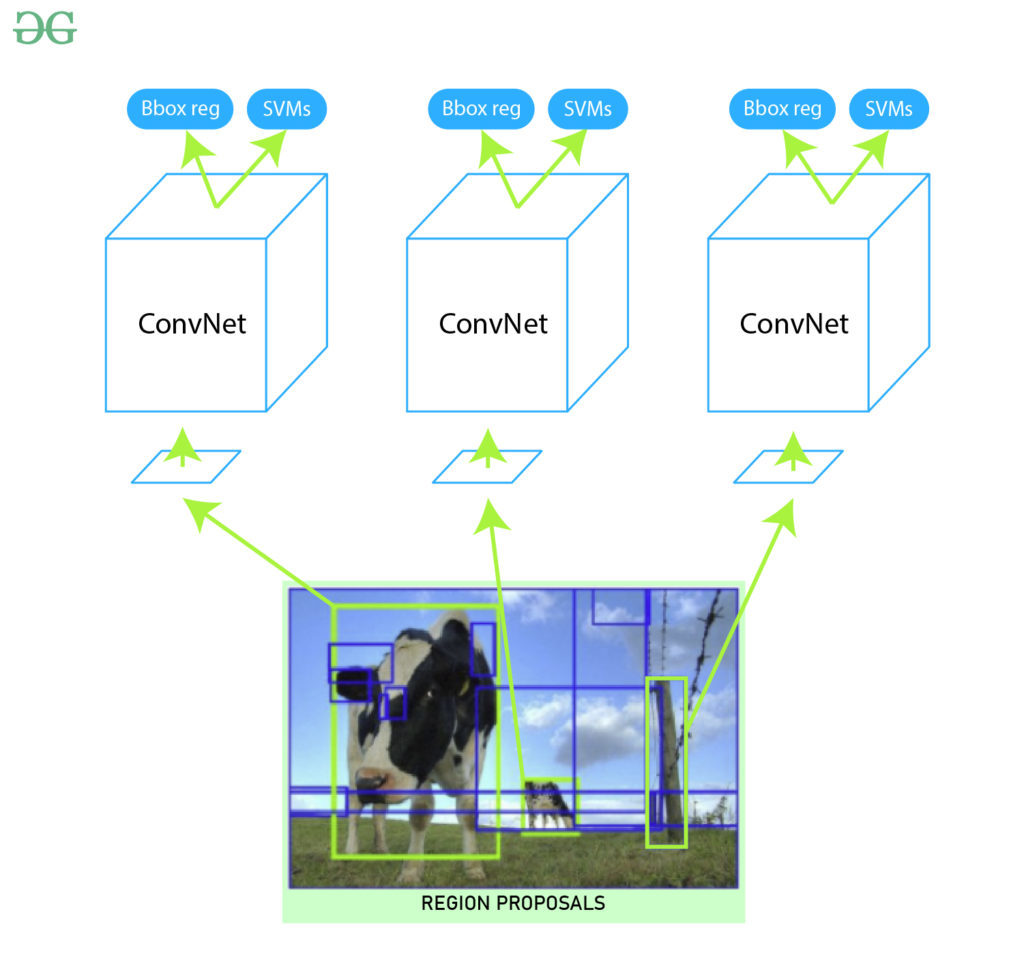
\includegraphics[width=\linewidth, height=3cm, keepaspectratio]{Pictures/convolutional-neural-network/rcnn-region-proposals.jpg}
            \caption*{RCNN: Region Proposals}
        \end{figure}        
    \end{minipage}
    \hfill
    \begin{minipage}[t]{0.49\linewidth}
        \begin{enumerate}
            \item Region proposals are simply the smaller regions of the image that possibly contains the objects we are searching for in the input image.
        
            \item To reduce the region proposals in the R-CNN uses a greedy algorithm called \textbf{selective search} (SEE: \fullref{Selective Search (CNN)}).
        \end{enumerate}
    \end{minipage}
\end{table}


\subsection{Bounding Box Regressor (BB-regression) \cite{https://www.geeksforgeeks.org/r-cnn-region-based-cnns/}}\label{Bounding Box Regressor (BB-regression)}

\begin{enumerate}
    \item In order to precisely locate the bounding box in the image, we used a scale-invariant linear regression model called \textbf{bounding box regressor}.

    \item For training this model we take as predicted and Ground truth pairs of four dimensions of localization.\\
    These dimensions are $(x, y, w, h)$ where:
    \begin{enumerate}
        \item $x$ and $y$ are the pixel coordinates of the center of the bounding box respectively. 

        \item $w$ and $h$ represent the width and height of bounding boxes.
    \end{enumerate}
    
    \item This method increases the \textbf{Mean Average precision (mAP)} of the result by $3-4\%$.
    
\end{enumerate}



\subsection*{Output}
\begin{enumerate}
    \item Now we have region proposals that are classified for every class label. 
    
    \item In order to deal with the extra bounding box generated by the above model in the image, we use an algorithm called \textbf{Non-maximum suppression} (SEE: \fullref{Non-maximum Suppression (NMS)}).\\
    It works in 3 steps:
    \begin{enumerate}
        \item Discard those objects where the confidence score is less than a certain threshold value(say $0.5$).

        \item Select the region which has the highest probability among candidates regions for the object as the predicted region.

        \item In the final step, we discard those regions which have \textbf{IoU (intersection Over Union)} (SEE: \fullref{IOU (Intersection over Union)}) with the predicted region over $0.5$.

    \end{enumerate}
\end{enumerate}

\subsection*{Challenges}
\begin{enumerate}
    \item Since there are approximately 2000 candidate proposals. It takes a lot of time to train the network. Also, we need to train multiple steps separately (CNN architecture, SVM model, bounding box regressor). So, This makes it very slow to implement.

    \item \textbf{R-CNN} (SEE: \fullref{Region Based CNNs (R-CNN/ RCNN)}) cannot be used in real-time because it takes approximately 50 sec to test an image with a bounding box regressor.

    \item Since we need to save feature maps of all the region proposals. It also increases the amount of disk memory required during training.
\end{enumerate}











\section{Fast R-CNN (2015) \cite{arxiv/1504.08083-fast-rcnn,medium/towardsdatascience.com/fast-r-cnn-for-object-detection-a-technical-summary-a0ff94faa022}}\label{Fast R-CNN}

\begin{figure}[h]
    \centering
    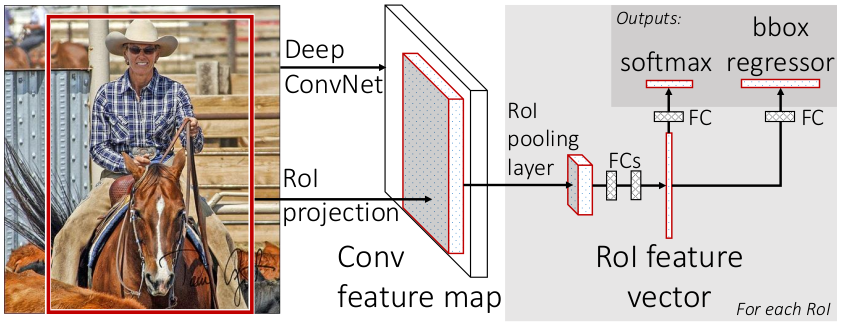
\includegraphics[width=\linewidth, height=3cm, keepaspectratio]{Pictures/convolutional-neural-network/fast-rcnn-arch.png}
    \caption*{Fast-RCNN: Architecture \cite{arxiv/1504.08083-fast-rcnn}}
\end{figure}

\begin{enumerate}
    \item The Fast R-CNN consists of a CNN (usually pre-trained on the ImageNet classification task) with its final pooling layer replaced by an “ROI pooling” layer and its final FC layer is replaced by two branches - a $(K + 1)$ category \textbf{softmax layer}(SEE: \fullref{Softmax function}) branch and a category-specific bounding box regression branch.

    \item The entire image is fed into the backbone CNN and the features from the last convolution layer are obtained. Depending on the backbone CNN used, the output feature maps are much smaller than the original image size. This depends on the stride of the backbone CNN, which is usually 16 in the case of a VGG backbone.

    \item The \textbf{object proposal windows} are obtained from a region proposal algorithm like \textbf{selective search} (SEE: \fullref{Selective Search (CNN)}). As explained in Regions with CNNs, object proposals are rectangular regions on the image that signify the presence of an object.

    \item The portion of the backbone feature map that belongs to this window is then fed into the \textbf{ROI Pooling layer} (SEE: \fullref{cnn: Region of Interest (ROI) Pooling Layer}).

    \item The output features from the ROI Pooling layer are then fed into the successive FC layers, and the softmax and BB-regression (SEE: \fullref{Bounding Box Regressor (BB-regression)}) branches. The softmax classification branch produces probability values of each ROI belonging to $K$ categories and one catch-all background category. The BB regression branch output is used to make the bounding boxes from the region proposal algorithm more precise.
\end{enumerate}

\subsection*{Loss}
\[
    \displaystyle
    L_{loc}(t^u, v) = \sum_{i \in \dCurlyBrac{x,y,w,h}} \operatorname{smooth}_{L_1}(t_i^u - v_i)
    \hfill
    \text{(For BB-Regression)}
\]
\[
    \displaystyle
    L(p,u,t^u,v) = L_{cls}(p,u) + \lambda[u\geq 1]L_{loc}(t^u, v)
    \hfill
    (\text{Multi-task loss})
\]

\noindent \textbf{Where},
\begin{customTableWrapper}{1.3}
\begin{table}[h]
    \begin{tabular}{l l}
        $K+1$ & Number of categories \\ \hline

        $p_i$ & Category ($i=0,\cdots,K$) \\
        $u$ & true class ($0/1$) \\ \hline

        $v$ & ground truth bounding box \\
        $t^u = (t^u_x,t^u_y,t^u_w,t^u_h)$ & predicted bounding box \\ \hline

        $L_{cls}(p,u) = -\log(p_u)$ & Classification loss \\
        $L_{loc}(t^u,v)$ & localization loss \\
    \end{tabular}
\end{table}
\end{customTableWrapper}










\section{Faster R-CNN (2015) \cite{arxiv/1506.01497-faster-rcnn,gfg/faster-r-cnn-ml}}\label{Faster R-CNN}

\url{https://www.geeksforgeeks.org/faster-r-cnn-ml/}\\
\url{https://arxiv.org/abs/1506.01497}





























\section{AnyNet Design Space \cite{dnn-1}} \label{AnyNet Design Space}

\begin{table}[H]
    \begin{minipage}{0.48\linewidth}
        \begin{figure}[H]
            \centering
            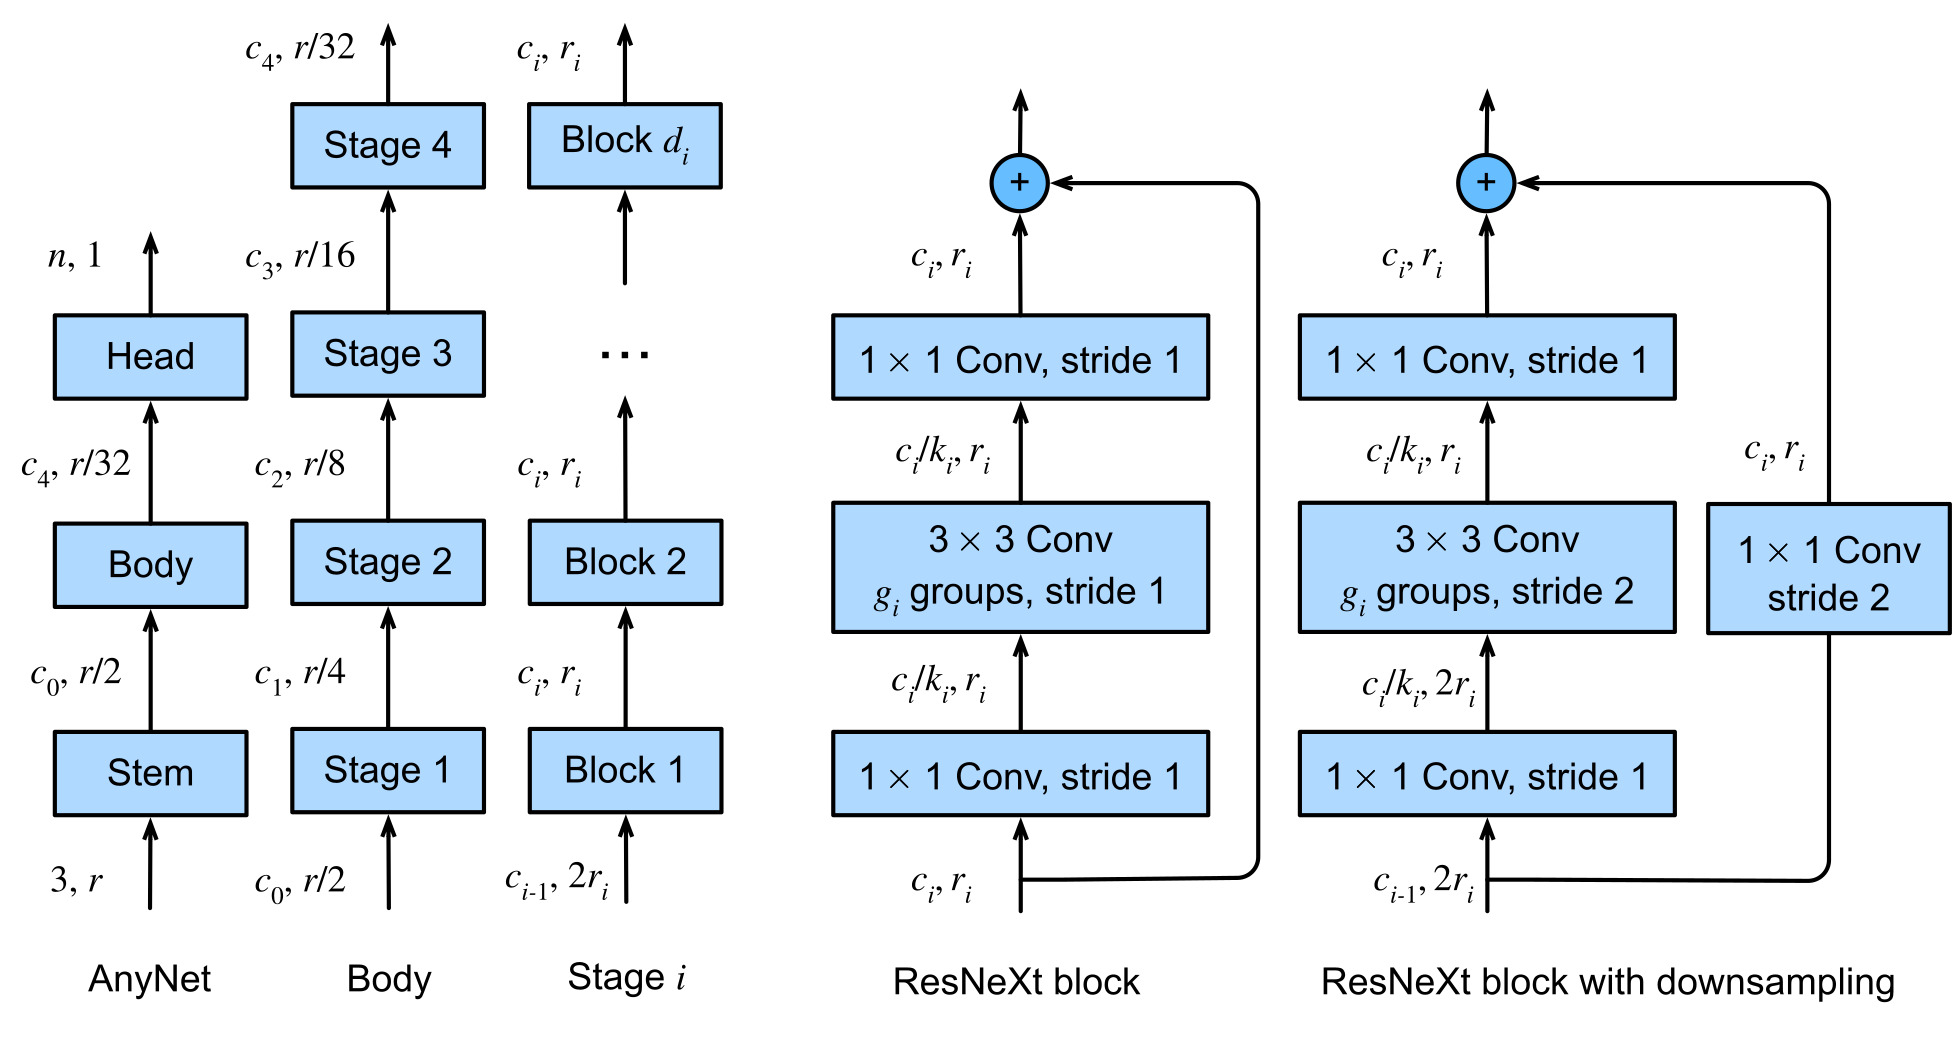
\includegraphics[width=\linewidth, height=5cm, keepaspectratio]{Pictures/convolutional-neural-network/anynet.jpg}
            \caption{The AnyNet design space}
        \end{figure}
    \end{minipage}
    \hfill
    \begin{minipage}{0.48\linewidth}
        \begin{customTableWrapper}{1.5}
            \begin{table}[H]
                \centering
                \begin{tabular}{l p{6cm}}
                    $(c,r)$ & number of channels and resolution $\mathit{r} \times \mathit{r}$ \\
                    
                \end{tabular}
            \end{table}
        \end{customTableWrapper}
        left to right:
        \begin{enumerate}
            \item generic network structure composed of stem, body, and head
            \item body composed of four stages
            \item detailed structure of a stage
            \item two alternative structures for blocks, one without downsampling and one that halves the resolution in each dimension. 
        \end{enumerate}

        Design choices include depth $\mathit{d_i}$, the number of output channels $\mathit{c_i}$, the number of groups $\mathit{g_i}$, and bottleneck ratio $\mathit{k_i}$ for any stage $i$
    \end{minipage}
\end{table}




\begin{enumerate}
    \item we need a template for the family of networks to explore

    \item the networks consist of a stem, a body and a head.
    \begin{enumerate}
        \item \textbf{stem}:
        \begin{enumerate}
            \item The {stem} performs initial image processing, often through convolutions with a larger window size.

            \item The stem takes as its input RGB images (3 channels), using a $3 \times 3$ convolution with a stride of $2$, followed by a batch norm, to halve the resolution from $r \times r$ to $r/2 \times r/2$

        \end{enumerate}

        \item \textbf{Body}
        \begin{enumerate}
            \item The \textbf{body} consists of multiple blocks, carrying out the bulk of the transformations needed to go from raw images to object representations.

            \item consists of multiple stages, operating on the image at decreasing resolutions.

            \item Most of the relevant design decisions are inherent to the body of the network. 
            
            \item It proceeds in stages, where each stage is composed of the same type of ResNeXt blocks

            \item The design there is again entirely generic: we begin with a block that halves the resolution by using a stride of $2$

            \item To match this, the residual branch of the ResNeXt block needs to pass through a $1 \times 1$ convolution. 
            
            \item This block is followed by a variable number of additional ResNeXt blocks that leave both resolution and the number of channels unchanged.

            \item a common design practice is to add a slight bottleneck in the design of convolutional blocks. As such, with bottleneck ratio $k_i \geq 1$ we afford some number of channels, $c_i/k_i$, within each block for stage $i$ (as the experiments show, this is not really effective and should be skipped).

            \item since we are dealing with ResNeXt blocks, we also need to pick the number of groups $g$ for grouped convolutions at stage $i$.

        \end{enumerate}

        \item \textbf{Head}
        \begin{enumerate}
            \item the \textbf{head} converts this into the desired outputs, such as via a softmax regressor for multiclass classification.

            \item the head employs an entirely standard design via global average pooling, similar to NiN, followed by a fully connected layer to emit an  $n$-dimensional vector for $n$-class classification

        \end{enumerate}

        \item both the stem and each subsequent stage quarter the spatial resolution

        \item each stage consists of one or more blocks

    \end{enumerate}
\end{enumerate}

\subsection{Distributions and Parameters of Design Spaces}

\begin{enumerate}[itemsep=0.15cm]
    \item parameters of a design space are hyperparameters of networks in that design space

    \item A better strategy would be to try to determine general guidelines of how the choices of parameters should be related. For instance, the bottleneck ratio, the number of channels, blocks, groups, or their change between layers should ideally be governed by a collection of simple rules.

    \item The approach in Radosavovic et al. (2019) relies on the following four assumptions:
    \begin{enumerate}
        \item We assume that general design principles actually exist, so that many networks satisfying these requirements should offer good performance. \\
        Consequently, identifying a distribution over networks can be a sensible strategy. \\
        In other words, we assume that there are many good needles in the haystack.

        \item We need not train networks to convergence before we can assess whether a network is good.\\
        Instead, it is sufficient to use the intermediate results as reliable guidance for final accuracy.\\
        Using (approximate) proxies to optimize an objective is referred to as multi-fidelity optimization (Forrester et al., 2007).\\
        Consequently, design optimization is carried out, based on the accuracy achieved after only a few passes through the dataset, reducing the cost significantly.

        \item Results obtained at a smaller scale (for smaller networks) generalize to larger ones.\\
        Consequently, optimization is carried out for networks that are structurally similar, but with a smaller number of blocks, fewer channels, etc.\\
        Only in the end will we need to verify that the so-found networks also offer good performance at scale.

        \item Aspects of the design can be approximately factorized so that it is possible to infer their effect on the quality of the outcome somewhat independently. \\
        In other words, the optimization problem is moderately easy.

    \end{enumerate}

    \item we can sample uniformly from the space of configurations and evaluate their performance. 
    
    \item Subsequently, we can evaluate the quality of the choice of parameters by reviewing the distribution of error/accuracy that can be achieved with said networks. 
    
    \item Denote by $F(e)$ the cumulative distribution function (CDF) for errors committed by networks of a given design space, drawn using probability disribution $p$. That is,
    \[
        \hfill
        F(e, p) \stackrel{\textrm{def}}{=} P_{\textrm{net} \sim p} \{e(\textrm{net}) \leq e\}
        \hfill
    \]

    \item Our goal is now to find a distribution $p$ over networks such that most networks have a very low error rate and where the support of $p$ is concise.\\
    Of course, this is computationally infeasible to perform accurately. 
    
    \item We resort to a sample of networks $\mathcal{Z} \stackrel{\textrm{def}}{=} \{\textrm{net}_1, \ldots \textrm{net}_n\}$ (with errors $e_1, \ldots, e_n$, respectively) from $p$ and use the empirical CDF $\hat{F}(e, \mathcal{Z})$ instead:
    \[
        \hfill
        \hat{F}(e, \mathcal{Z}) = \dfrac{1}{n}\dsum_{i=1}^n \mathbf{1}(e_i \leq e)
        \hfill
    \]

    \item Whenever the CDF for one set of choices majorizes (or matches) another CDF it follows that its choice of parameters is superior (or indifferent).

    \item[] 
    \begin{customTableWrapper}{1.5}
    \begin{longtable}{l p{10cm}}
        $\textrm{AnyNet}_\mathit{A}$ & original design space \\
    
        $\textrm{AnyNet}_\mathit{B}$ & ties the bottleneck ratios \\
    
        $\textrm{AnyNet}_\mathit{C}$ & also ties group widths \\
    
        $\textrm{AnyNet}_\mathit{D}$ & increases the network depth across stages \\
    \end{longtable}
    \end{customTableWrapper}

\subsection{AnyNetX series \cite{dnn-1}}
    \item $\textrm{AnyNetX}_D$
    \begin{enumerate}
        \item It is a reasonable assumption that, as we go deeper, the number of channels/ width should increase, i.e., $c_i \geq c_{i-1}$ (or, $w_{i+1} \geq w_i$), yielding $\textrm{AnyNetX}_D$.
    \end{enumerate}

    \item $\textrm{AnyNetX}_E$
    \begin{enumerate}
        \item it is equally reasonable to assume that as the stages progress, they should become deeper, i.e., $d_i \geq d_{i-1}$, yielding $\textrm{AnyNetX}_E$
    
        \item The resulting $\textrm{AnyNetX}_E$ design space consists of simple networks following easy-to-interpret design principles:
        \begin{enumerate}
            \item Share the bottleneck ratio $k_i = k$ for all stages $i$
    
            \item Share the group width $g_i = g$ for all stages $i$
    
            \item Increase network width across stages: $c_{i} \leq c_{i+1}$
    
            \item Increase network depth across stages: $d_{i} \leq d_{i+1}$
    
        \end{enumerate}

        \item the width of the network ideally increases linearly with the block index across the network, i.e., $c_j \approx c_0 + c_a j$, where $j$ is the block index and slope $c_a > 0$. 
        
        \item Given that we get to choose a different block width only per stage, we arrive at a piecewise constant function, engineered to match this dependence. 
        
        \item Furthermore, experiments also show that a bottleneck ratio of $k = 1$ performs best, i.e., we are advised not to use bottlenecks at all.

        
    \end{enumerate}



\end{enumerate}


\section{RegNet \cite{dnn-1}} \label{RegNet}

SEE: $\textrm{AnyNetX}_E$ \fullref{AnyNet Design Space}

\begin{enumerate}[itemsep=0.15cm]
    \item 32-layer RegNetX variant
    \begin{enumerate}
        \item $k = 1$ (no bottleneck)
        \item $g = 16$ (group width is 16)
        \item $c_1 = 32$ and $c_2 = 80$ channels for the first and second stage, respectively
        \item $d_1=4$ and $d_2=6$ blocks deep

    \end{enumerate}

    \item RegNetX even holds for Squeeze-and-Excitation (SE) network designs (RegNetY) that have a global channel activation

\end{enumerate}

















































































































